\chapter{Hydrometeorological controls on landscape erosion and evolution}
\label{chapter_hydrogeomorph}
\chaptermark{Hydrometeorological controls on landscape erosion}

\section{Introduction}

Landscape evolution is punctuated by intense erosive episodes driven by flood events triggered by intense rainfall \citep{Wolman1960,newson1980geomorphological,Costa1995}. Understanding the role rainfall plays in erosional processes is of importance to both long-term landscape evolution studies \citep[e.g.][]{rinaldo1995geomorphological,tucker1997drainage,Tucker2000}, which have long sought effective ways of parameterising rainfall patterns within models \citep[e.g][]{Eagleson1978}.  Catchment sensitivity to rainfall variability is also important in the context of environmental prediction, such as predicting the likely geomorphological impacts of intense rainfall and flash flood events \citep[e.g.][]{lane2007interactions,deluis2010rainfall,milan2012geomorphic}. Given the possibility of changing hydro-meteorological conditions that may accompany climate change \citep{Kendon2014}, longer-term prediction of catchment sediment yields and erosion patterns has also seen an increased research effort in recent years \citep{coulthard2000modelling,Coulthard2012,hancock2017sediment}, The drive to understand how landscapes respond to climatic conditions is aided greatly through the use of numerical landscape evolution models \citep{Tucker2010}, which allow a wide range of scenarios to be tested, and quantify the sensitivity of particular processes to climatic boundary conditions, including rainfall distribution.

Investigation into infrequent but geomorphologically formative flash flooding events has seen a resurgence by recent work such as \citet{Huang2006}, looking at the long-term implications of different geomorphically effective event discharges on fluvial incision. Other studies have sought to quantify the amount of bedrock erosion during individual large flood events \citep[e.g.][]{gupta2007catastrophic,lamb2010rapid,baynes2015erosion}, in an effort to better understand the role that low frequency, but high magnitude events have on landscape evolution. Still, our understanding of catchment-scale landscape evolution is far from complete -- the role that rainfall plays in individual events appears to be highly variable from case-to-case. The behaviour of streams and rivers within catchments can vary in response to the same magnitude of flood event -- some streams may erode during high flows, whereas others may deposit during high flows \citep{turowski2013large}. During small--medium flows \citet{turowski2013large} also report that the dynamics of erosion are is reversed, with some rivers acting as agents of deposition during floods, rather than being primarily erosional, depending on the preconditioning of the catchment by previous events. Further studies have reported that rapid gorge formation can be driven primarily by small to moderate sized floods \citep{anton2015exceptional}, rather than rainfall events of much larger magnitude.

Temporal variability in rainfall patterns is shown to control the evolution of landscapes over geological timescales, with the ability to influence the geomorphology of drainage basins and geometry of channel networks \citep{Tucker2000,Solyom2004}. The influence of spatial variability in rainfall patterns has also been shown to affect the outcome of long-term topographic evolution, creating distinct topographic signatures in landscapes subject to orogoraphic rainfall gradients \citep{solyom2007importance,han2014modeling,han2015measuring}. Sediment yields and morphological change have also been shown to be sensitive to the resolution of rainfall inputs over decadal to millenial timescales \citep{coulthard2016sensitivity}. However, no study has yet looked at the sensitivity of erosion to rainfall spatial patterns during single storm events -- the goal of this chapter is to investigate the potential sensitivity of catchment-scale erosional processes to spatially distributed rainfall inputs.

% A clear relationship between rainfall intensity, flood magnitude, and erosional dynamics is not always observed in case studies (Anton 2012), suggesting that the links between precipitation, hydrological response, and sediment transport are not yet fully understood.
%
%The behaviour of certain catchment processes also exhibits non-linearity in response to external forcings \citep{coulthard1998non,coulthard2007cellular}, which suggests why case studies do not always exhibit a clear scaling relationship between event magnitude and catchment response. T  Catchment-scale erosional dynamics are complex, and except in the simplest cases depend on other forcings other than the magnitude of single flood events alone.  The understanding of hydrogeomorphic processes during single storm events is not only important for the long-term evolution of landscapes, 

% More detail
\subsection{Theory}
The assumption of uniform rainfall over a river catchment is argued to hold true for small catchments \citep{Solyom2004,Tucker2010}, but even over small areas, mesoscale rainfall features, such as localised convective storm cells, can result in spatially and temporally uneven input of precipitation into the catchment \citep{Peleg2014}. In the case of intense convective precipitation, individual storm cells can be as small as 10km$^2$ in areal extent  \citep{weisman1986characteristics,vonhardenberg2003shape}. Over larger catchments, or those with steep topographic gradients, precipitation is likely to vary spatially, due to orographic enhancement of rainfall \citep{Roe2003,han2015measuring}. As such, rainfall-runoff generation, local river and tributary discharge, and erosion rates may vary considerably within individual drainage basins. 

As discussed in Chapter \ref{chapter_landscape_evol}, current numerical models of landscape evolution usually omit a realistic distribution of rainfall input in favour of uniform, homogenised precipitation across the landscape. When precipitation is `lumped', either spatially or temporally in a catchment, local minima and maxima of precipitation are lost or smoothed-out. With discharge being a function of rainfall rate, this smoothing should therefore be expected to propagate through to local discharges and erosion rates. The uncertainty in erosion rates is potentially exacerbated by the non-linearity and threshold dependence of erosive processes \citep{coulthard1998non,phillips2003sources}. The variability of precipitation is considered to be as important as total precipitation amount in determining erosional effectiveness \citep{Tucker2000,Tucker2010}. As many geomorphic processes are threshold dependent \citep{schumm1979geomorphic}, such as fluvial incision into bedrock \citep{sklar2001sediment,snyder2003importance}, there is potential for the spatial distribution of rainfall to control local erosion rates within a catchment. 
%Non-linearity in geomorphic process laws \citep{coulthard1998non,phillips2003sources,coulthard2007cellular} should dictate that catchments are also geomorphically sensitive to the spatial distribution of rainfall. 

Rainfall resolution has been demonstrated to exert a control over sediment yields over decadal and millennial timescales \citep{coulthard2016sensitivity}. In a numerical modelling study of the River Swale catchment, UK, \citet{coulthard2016sensitivity} show that local distribution of erosion differed and catchment-wide sediment yields were predicted to increase by up to 100\% as rainfall data resolution was increased. The study looked at the effects of rainfall input data grid-spacing as well the temporal resolution of rainfall data, showing both to have a control over sediment erosion within the catchment. The results were based on landscape evolution model simulations over a period of 1000 years, rather than individual storm events.

In numerical models of landscape evolution, resolving the precise temporal and spatial details of rain storms and the hydrological response is often computationally prohibitive, especially over long timescales, and as such modellers have taken to using simpler parameterisiations of storm characteristics, such as using simple stochastic models to generate rainfall inputs and rainfall timeseries \citep{Eagleson1978,Tucker2001}. In Chapter \ref{chapter_HAIL-CAESAR}, an existing landscape-evolution model was redeveloped to address some of the computational issues and make it suitable for deployment on a high-performance computing service, enabling more effective use of higher resolution digital topography data to initialise the terrain surface (Chapter \ref{chapter_events}) and finer-resolution rainfall input data to drive the model.

\subsection{Objectives}
The aim of this chapter is to assess how erosional processes are sensitive to the details of precipitation across a catchment during individual storms. The focus in this study is to quantify the sensitivity of erosional processes to the spatial distribution of rainfall during flood events, using the case studies outlined in Chapter \ref{chapter_events}.

The following questions are explored through the use of numerical modelling simulations:

\begin{enumerate}
\item Are fluvial erosion and sediment transport processes sensitive to the details of precipitation distribution at the catchment scale during single storm events?
\item Does the choice of erosional model operating within the catchment influence sensitivity to rainfall patterns? 
\item What are the implications of this for longer term landscape evolution? 
\end{enumerate}

%The hypothesis for this chapter can be summarised (as in Chapter \ref{chapter_events}, Section \ref{section_experiment_design}) as follows:
%
%\begin{enumerate}
%\item \label{itm:geomorph} \textbf{Erosional processes in river catchments are sensitive to the spatial distribution of rainfall inputs.}
%  \begin{enumerate}
%  \item Erosion and sediment transport processes are sensitive to thresholds determining erosion initiation and sediment entrainment.   holds true, then fluvial erosional processes should exhibit sensitivity to the spatial distribution of rainfall inputs of rainfall as well.
%  \item The parameterisation of erosional processes in the model also determines the spatial pattern of erosion and deposition, but does spatial variation in rainfall inputs exert a greater control than the choice of erosion law?
%  \end{enumerate}
%\end{enumerate}

To build upon the work done in previous studies \citep[e.g.][]{han2014measuring, coulthard2016sensitivity}, this chapter focuses on the sensitivity of sediment yield and erosion distribution to rainfall heterogeneity at timescales not previously investigated -- single severe rain storms. 
%Landscape response is investigated using a numerical landscape evolution model that incorporates a dynamic water-routing component \citep{bates2010simple} and a range of fluvial erosion and sediment transport laws \citep{howard1983channel,wilcock2003surface,whipple1999dynamics}. 
Results from series of numerical simulations set out in Chapter \ref{chapter_events} are presented to assess how sensitive real landscapes are to the catchment-scale details of precipitation during intense rainfall events. The simulations are each based on selected severe storms in the UK occurring in the past decade, which left significant flooding, damage, and geomorphological change in their wake (Chapter \ref{chapter_events}).

%\section{Experiment design}
%
%\begin{table}
%\begin{tabular}{lll}
%\\
%\textbf{Experiment name}   & \textbf{Rainfall input} & \textbf{Erosion law}  \\
%\hline
%UNIFORM\_DLIM      &  Spatially-averaged Radar   & Detachment-limited \\
%UNIFORM\_TLIM       &  Spatially-averaged Radar  & Transport-limited \\
%
%GRIDDED\_DLIM      &  1km Radar Gridded  & Detachment-limited \\
%GRIDDED\_TLIM       &  1km Radar Gridded  & Transport-limited \\
%\hline \\ 
%\end{tabular} 
%\caption{Summary of the subset of model simulations carried out for both the Ryedale and Boscastle case studies, simulating erosional processes within the catchment.}
%\label{table_ensemble_experiments_erosion}
%\end{table}

\section{Results}

Sediment flux predictions are presented at a catchment-wide scale, measured from the outlet of each catchment (Figures \ref{fig_boscastle_sedigraph_ensemble}, \ref{fig_ryedale_sedigraph_ensemble}). The spatial distribution of sediment deposition is presented in the form of 1D longitudinal profiles along the main channel (Figures \ref{fig_boscastle_swath_tlim}, \ref{fig_ryedale_swath_tlim}), as well as 2D planform maps of erosion and deposition distribution (Figures \ref{fig_boscastle_erodediff_grid_tlim}, \ref{fig_boscastle_erodediff_uniform_tlim}, \ref{fig_boscastle_2dplan_erosion_ensemble}, \ref{fig_boscastle_2dplan_erosion_ensemble_SE}, \ref{fig_ryedale_2dplan_erosion_ensemble})

\subsection{Catchment sediment flux}
% General description of all results.
%In contrast to water fluxes (Chapter \ref{chapter_flood_model_sensitivity}), 
Sediment flux from both catchments was found to be most sensitive to the sediment erosion parameterisation, rather than the spatial detail of rainfall inputs (Figures \ref{fig_boscastle_sedigraph_ensemble}, \ref{fig_ryedale_sedigraph_ensemble}). For both catchments simulated, sediment flux from each catchment was higher in the simulations using the transport-limited erosion law, by up to an order of magnitude. All detachment-limited simulations resulted in a much lower prediction in sediment fluxes.

The influence of rainfall input data spatial resolution played a secondary role in determining sediment yields. In almost simulations, when the same erosion law parameterisation was used, sediment yields were greater with gridded rainfall data input. The only exception was in the Boscastle detachment-limited simulations (\texttt{DLIM}), where sediment output was actually slightly lower with gridded rainfall input to the simulation (Figure \ref{fig_boscastle_sedigraph_ensemble}).

The patterns of peak sediment discharge also mirrored that of water discharge (see Chapter \ref{chapter_flood_model_sensitivity}), with sediment flux peaking earlier in the simulations with higher resolution rainfall inputs. 

\begin{figure}[t]
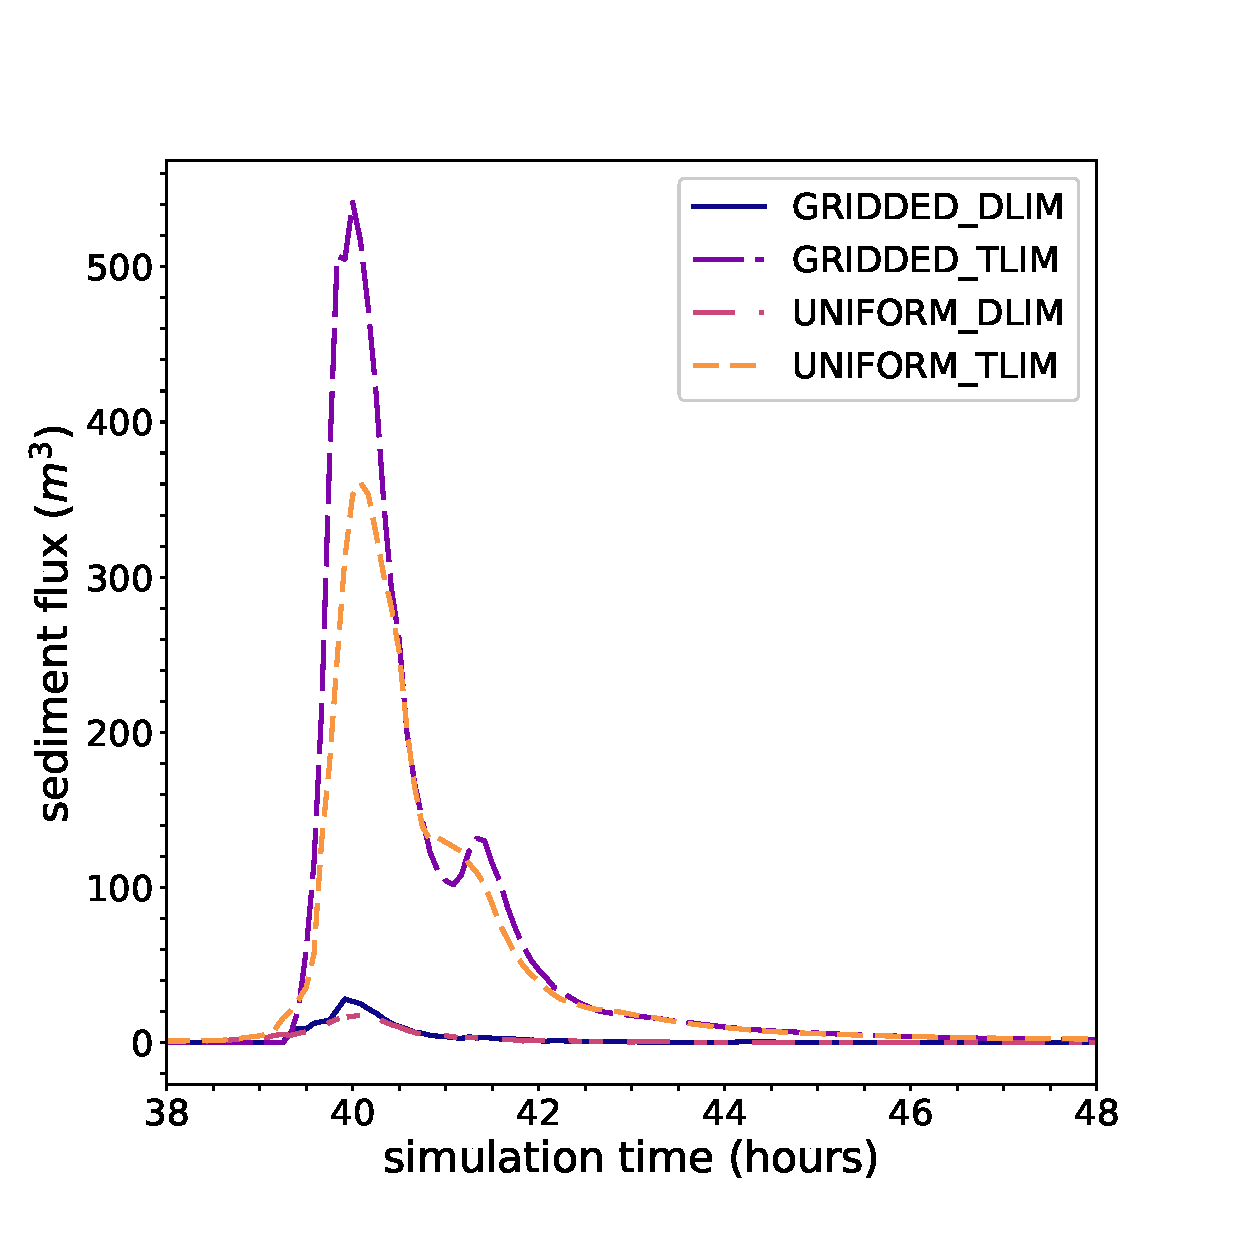
\includegraphics[width=14cm]{chp06_figures_scripts/figure_boscastle_sedigraph_ensemble.eps}
\caption{Boscastle sediment flux (total sediment volume output per hour at catchment outlet for each erosion-enabled simulation of the 2004 Boscastle event listed in Table \ref{table_ensemble_experiments}.}
\label{fig_boscastle_sedigraph_ensemble}
\end{figure}

\begin{figure}[t]
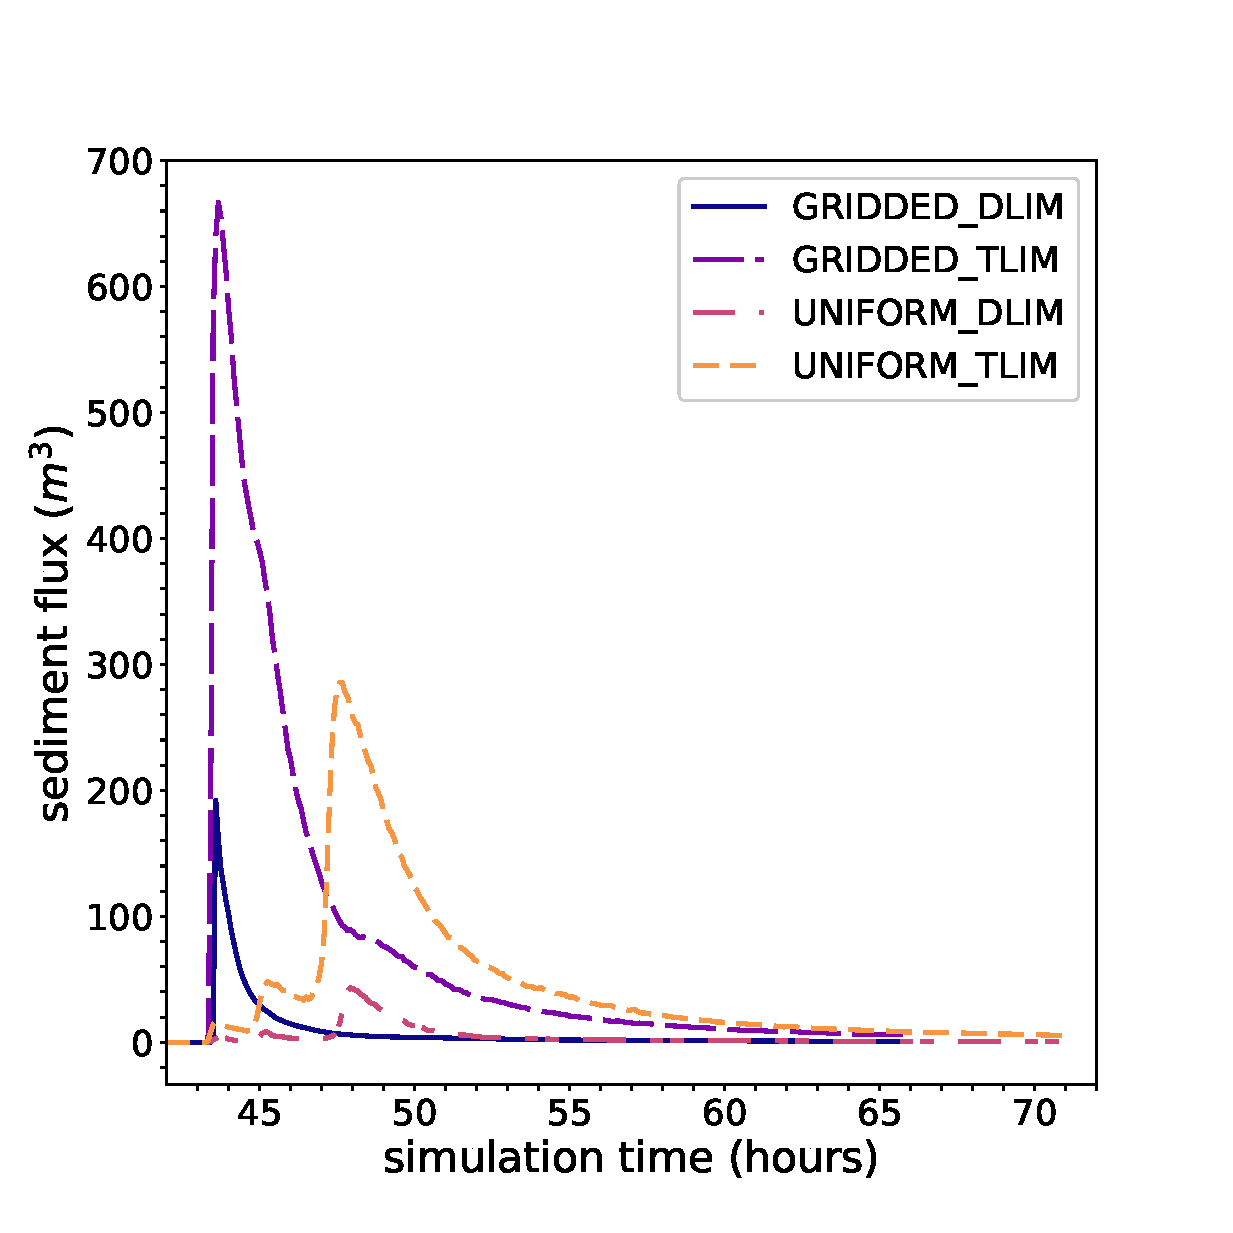
\includegraphics[width=14cm]{chp06_figures_scripts/figure_ryedale_sedigraph_ensemble.eps}
\caption{Ryedale sediment flux (Total sediment volume output per hour at catchment outlet) for each erosion-enabled simulation of the 2005 Ryedale event listed in Table \ref{table_ensemble_experiments}.}
\label{fig_ryedale_sedigraph_ensemble}
\end{figure}

% Describe planform variations in erosion and deposition
\subsection{Spatial variations in channel erosion}
The main spatial variation seen in sediment erosion is seen within river channels. The amount of erosion in each simulation was highly sensitive to parameterisation choice of the sediment erosion and transport law, with the choice of rainfall input data (gridded vs uniform) being only a secondary controlling factor on the spatial distribution of erosion, all other factors being equal. This behaviour was exhibited in all simulations, shown in Figures \ref{fig_boscastle_2dplan_erosion_ensemble} and \ref{fig_ryedale_2dplan_erosion_ensemble}.  As differences between the \texttt{GRIDDED} and \texttt{UNIFORM} simulations were minimal, and erosion amounts in the detachment-limited simulations were small, it was elected to only show the profiles from the \texttt{GRIDDED\_TLIM} for clarity.

To highlight the variation in erosion along the river channel, longitudinal channel profiles showing the average change in elevation after the storm are shown in Figures \ref{fig_boscastle_swath_tlim} and \ref{fig_ryedale_swath_tlim}. The longitudinal profile shows the variation in erosion along the main channel within each catchment, averaged over a 10m wide channel cross-section centred on the midpoint of the channel. The longitudinal profiling technique is adapted from \citep{hergarten2014extracting}, where the resulting profiles are termed \textit{swath} profiles. Originally the swath profiling technique was written to calculate cross-sectional profiles across mountain ranges or basins, but here it has been adapted to create longitudinal profiles. To reduce the number of points plotted along the swath profile, erosion is also averaged longitudinally, using bins spaced every 200m in the Rye river channel and every 50m in the Valency river channel.

% Swath profiles
% Boscastle TLIM
\begin{figure}[htb]
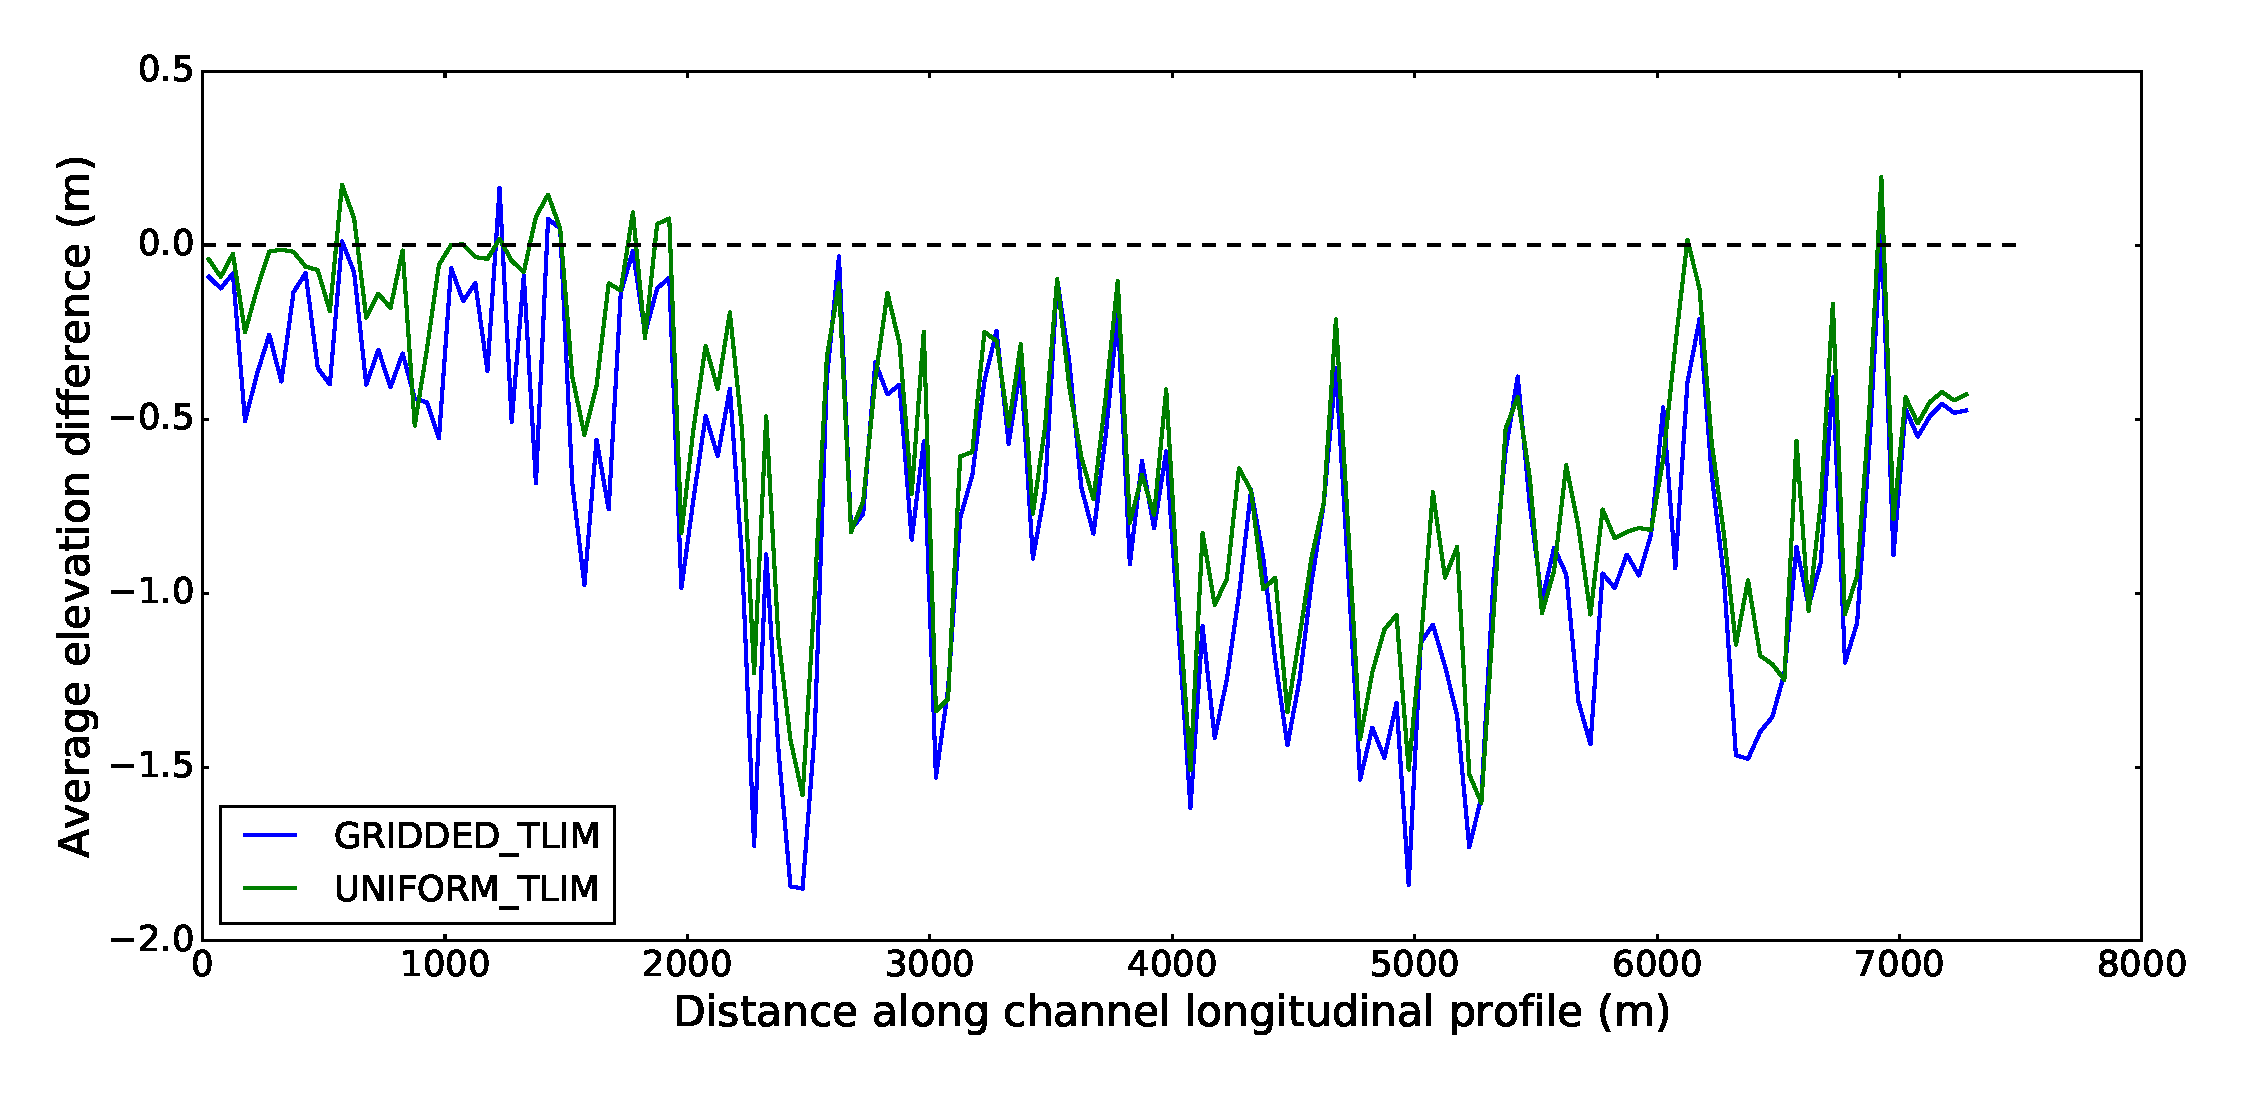
\includegraphics[width=14cm]{chp06_figures_scripts/fig_swath_profile_boscastle_erode_tlim.eps}
\caption{Channel averaged elevation difference along the main river channel in the Valency catchment. Simulation using the transport limited erosion parametrisation. Longitudinal profile is averaged over bins spaced every 50m. Transverse averaging (across the channel) is done over a 10m wide section centred on the channel midpoint. Results from the \texttt{GRIDDED\_TLIM} simulation shown in blue and the \texttt{UNIFORM\_TLIM} simulation shown in green.}
\label{fig_boscastle_swath_tlim}
\end{figure}

% Ryedale TLIM
\begin{figure}[htb]
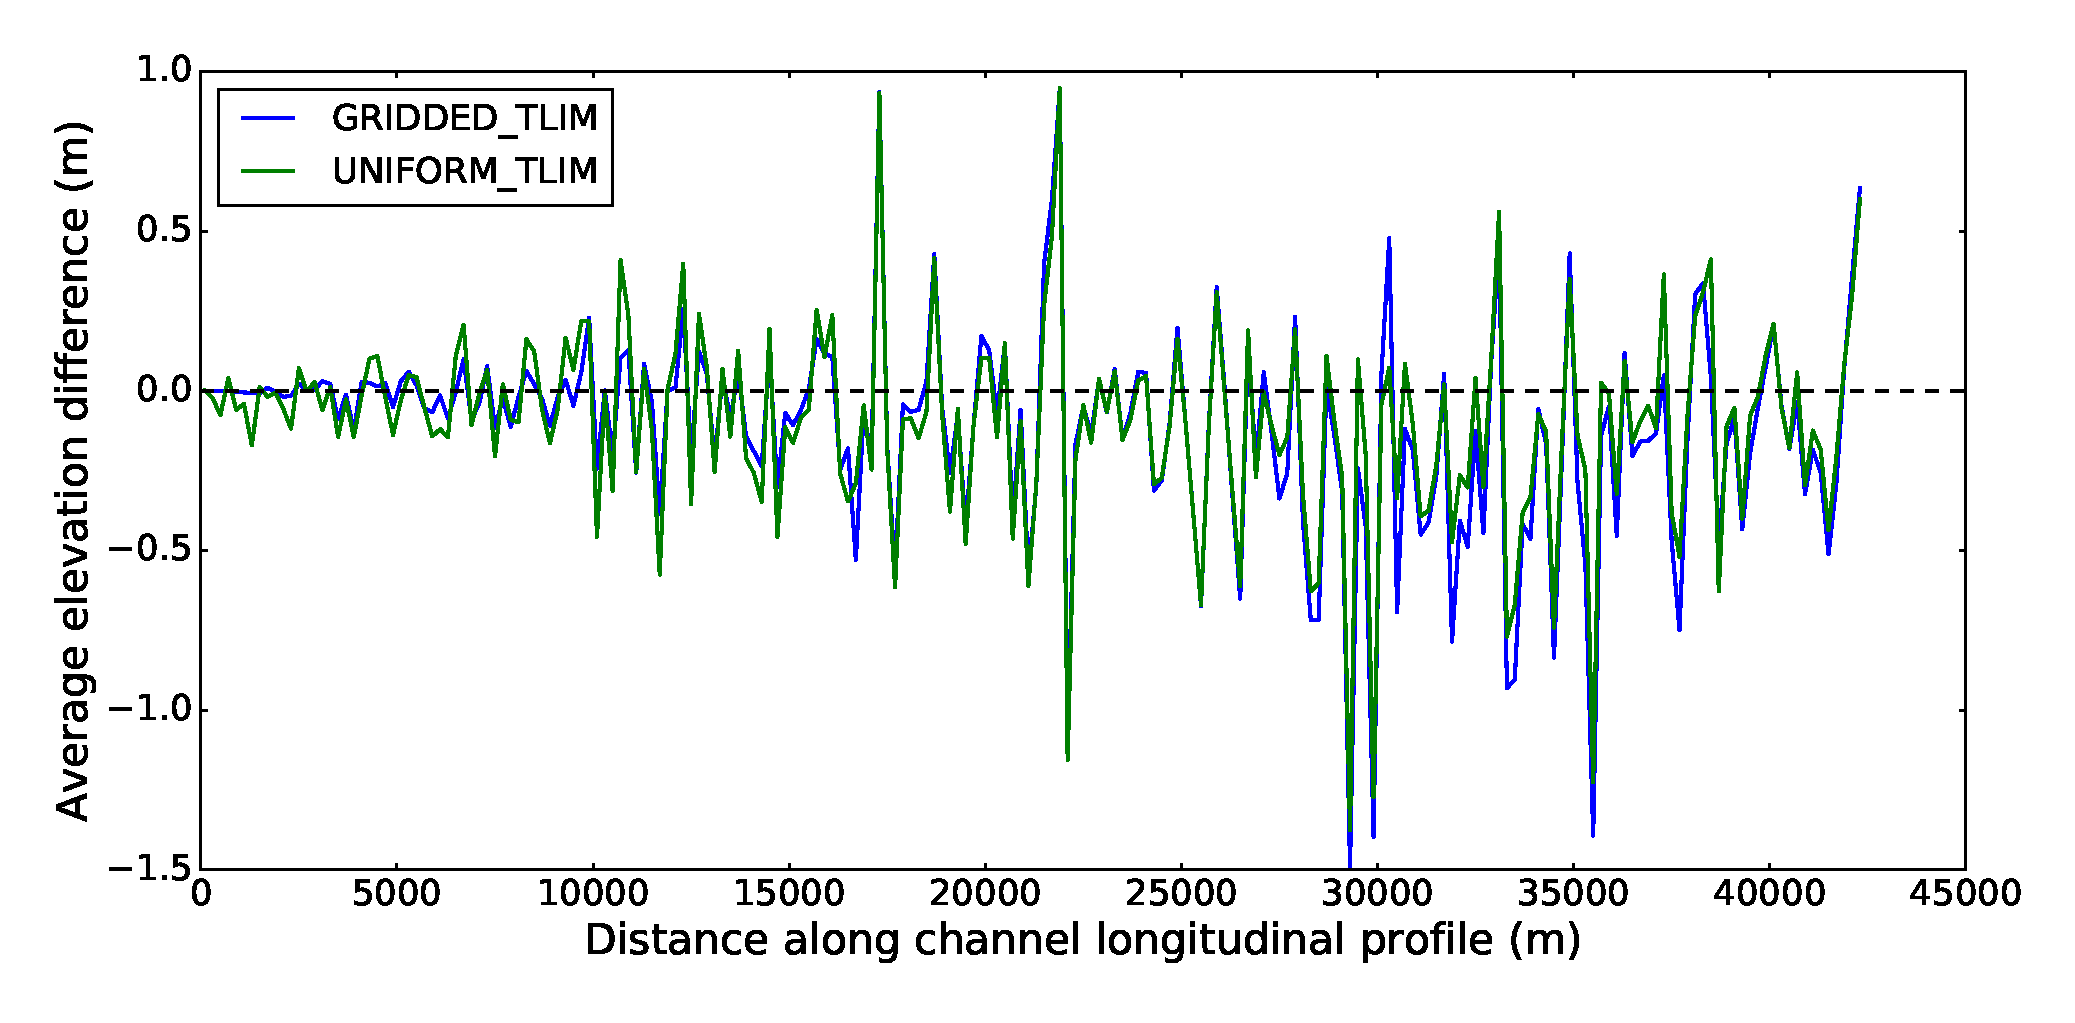
\includegraphics[width=14cm]{chp06_figures_scripts/fig_swath_profile_ryedale_erode_tlim.eps}
\caption{Channel averaged elevation difference along the main river channel in the Ryedale catchment. Simulation using the transport limited erosion parametrisation. Longitudinal profile is averaged over bins spaced every 200m. Transverse averaging (across the channel) is done over a 10m wide section centred on the channel midpoint. Results from the GRIDDED\_TLIM simulation shown in blue and the UNIFORM\_TLIM simulation shown in green.}
\label{fig_ryedale_swath_tlim}
\end{figure}

Swath profiling of the Valency river channel (Boscastle) shows overall net incision under transport-limited erosion parameterisation, with only small sections of the channel showing net sediment deposition (elevation increase) on average (Figure \ref{fig_boscastle_swath_tlim}. Most incision is predicted to occur in the mid to upper reaches of the channel, with relatively little incision in the lowest reach of the catchment. The difference between gridded and uniform rainfall inputs shows a minimal difference along the main profile, though there is a slight tendency for the incision seen in the gridded rainfall input simulation to be higher in most places than the simulation using uniform input, with the difference in incision amounts between gridded and uniform rainfall inputs being of the order of tens of centimetres.

The swath profiling of the Rye river channel shows a large variation in incision and deposition rates within the catchment, though there is an overall tendency for net incision (Figure \ref{fig_ryedale_swath_tlim}). The magnitude of both incision and deposition is higher in the mid to upper reaches of the Rye river channel, similar to the pattern observed in the Valency river. The differences in average elevation changes are not as clearly distinguishable between the gridded and uniform rainfall input parameterisations; magnitudes of erosional and depositional peaks are slightly higher in the lower reaches of the river channel, but in the mid to upper reaches the differences are more varied. 
 
% OTHER SWATH PROFILES? DLIM, WIDER SWATH HALF WIDTH PERHAPS FOR RYEDALE?????
%
%

% APPENDIX DISCUSSING SWATH PROFILE ALGO?

\subsection{Local variation in erosion patterns}

\subsubsection{General observations}
Though the choice of erosion law has a strong control on the \textit{amount} of sediment erosion, it does not appear to influence the \textit{distribution} of erosion over the catchment. Detachment-limited simulations exhibit a similar variation in spatial distribution of erosion, but overall with much lower amounts of incision and deposition. 

\subsubsection{Boscastle}
In the Boscastle catchment, there are slight differences in the spatial distribution of erosion between the gridded and uniform rainfall input simulations. In the area along the main channel of the Valency river around Boscastle village, gridded and uniform rainfall simulations appear to show very similar erosion and deposition amounts (Figure \ref{fig_boscastle_2dplan_erosion_ensemble}). The more obvious contrast lies in the choice of erosion law, with transport-limited erosion simulations predicting much higher amounts of elevation change.

In the south-eastern section of the catchment, the predicted amounts of erosion are notably higher in upper tributaries and adjacent hillslopes under the gridded rainfall simulation (Figure \ref{fig_boscastle_erodediff_grid_tlim}), when compared with the uniform rainfall input simulation (Figure \ref{fig_boscastle_erodediff_uniform_tlim}). In the smaller tributaries of the catchment, detachment-limited simulations predicted little or no erosion. Figure \ref{fig_boscastle_2dplan_erosion_ensemble_SE} shows the Lesnewth stream and the erosion/deposition amounts in each simulation. The highest levels of erosion and deposition are predicted by the gridded rainfall, transport-limited erosion case, and in contrast there is almost no erosion predicted by the uniform rainfall, detachment-limited erosion case.


\subsubsection{Ryedale}
In the Ryedale catchment, the gridded rainfall input simulations predict slightly greater amounts of erosion and deposition in general, though it is difficult to pick out a particular area of the catchment where the differences are starkly contrasting. The spatial distribution of erosion and deposition in the Helmsley area is shown in Figure \ref{fig_ryedale_2dplan_erosion_ensemble}, for each of the four simulations. Small differences can be seen along the main floodplain and up into the gorge area of the river Rye, showing elevated levels of erosion and deposition in the gridded rainfall input simulations. In contrast to the Boscastle simulations, there was comparatively little sediment transport shown in any of the hillslope areas -- compare the yellow shaded areas over the hillslopes in the Boscastle castchment erosion map (Figure \ref{fig_boscastle_erodediff_grid_tlim}) and their notable absence in the Ryedale catchment erosion map (Figure \ref{fig_boscastle_erodediff_grid_tlim}.
As with the Boscastle simulations, the most obvious contrast in erosion amounts is seen between the different erosion law simulations.


%Discuss 2d planform maps for better prep for discussion section afterwards.

% Plan view erosion diff maps
\begin{sidewaysfigure}[t]
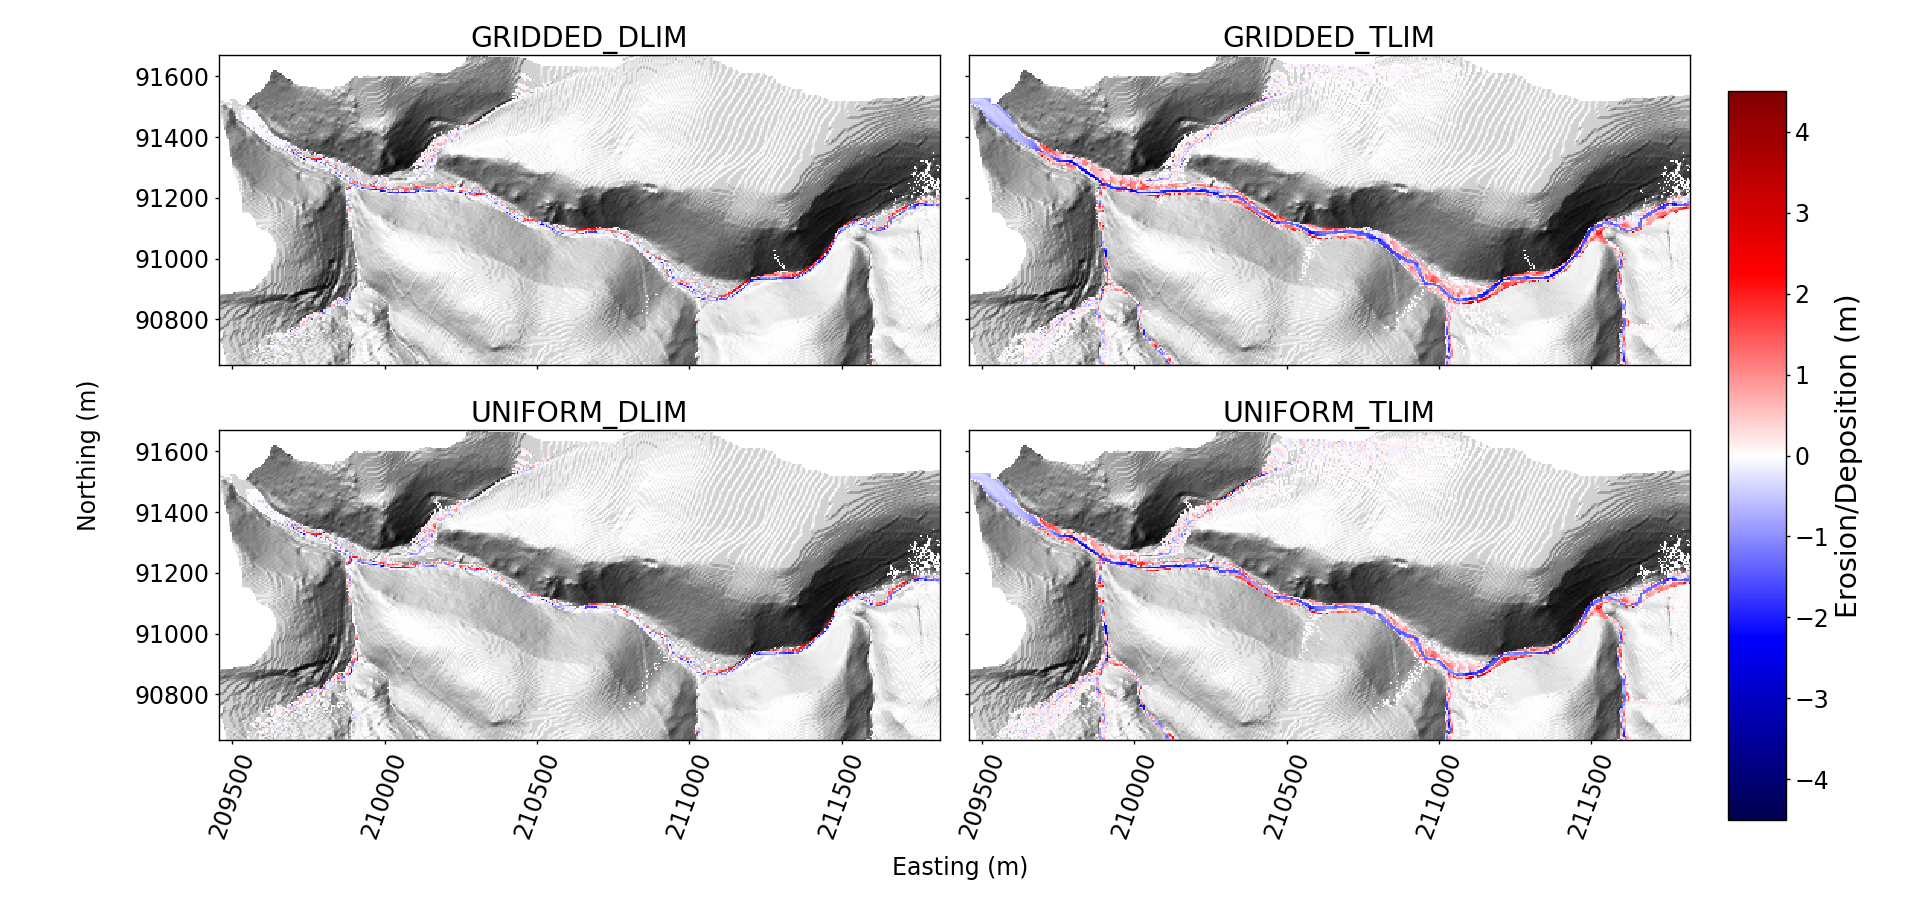
\includegraphics[width=25cm]{chp06_figures_scripts/figure_boscastle_erosion_diff_ensemble.png}
\caption{Boscastle. River Valency main channel in vicinity of Boscastle village. Net difference in elevation after 72 hours simulation, showing the gridded and uniform rainfall simulations, for each of the two erosion law end-members (transport-limited and detachment-limited). Elevation change smaller than \(\pm\) 0.2m in magnitude is not shown for clarity. Boscastle harbour is located in the upper left corner of each figure.}
\label{fig_boscastle_2dplan_erosion_ensemble}
\end{sidewaysfigure}

\begin{sidewaysfigure}[t]
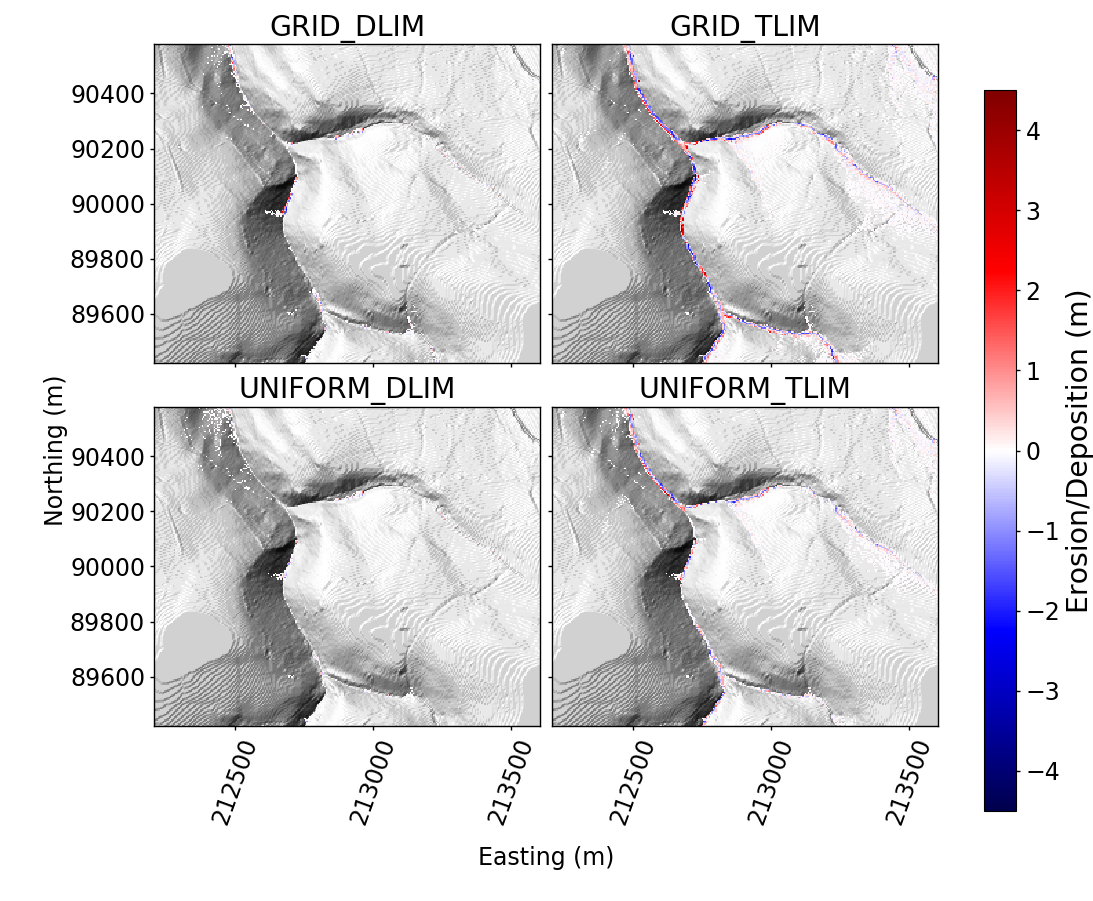
\includegraphics[width=18cm]{chp06_figures_scripts/figure_boscastle_erosion_diff_ensemble_SE.png}
\caption{Boscastle. South-east section of catchment showing the Lesnewth Stream tributary channel. Net difference in elevation after 72 hours simulation, showing the gridded and uniform rainfall simulations, for each of the two erosion law end-members (transport-limited and detachment-limited). Elevation change smaller than \(\pm\) 0.2m in magnitude is not shown for clarity. }
\label{fig_boscastle_2dplan_erosion_ensemble_SE}
\end{sidewaysfigure}

% Plan view erosion diff maps
\begin{sidewaysfigure}[t]
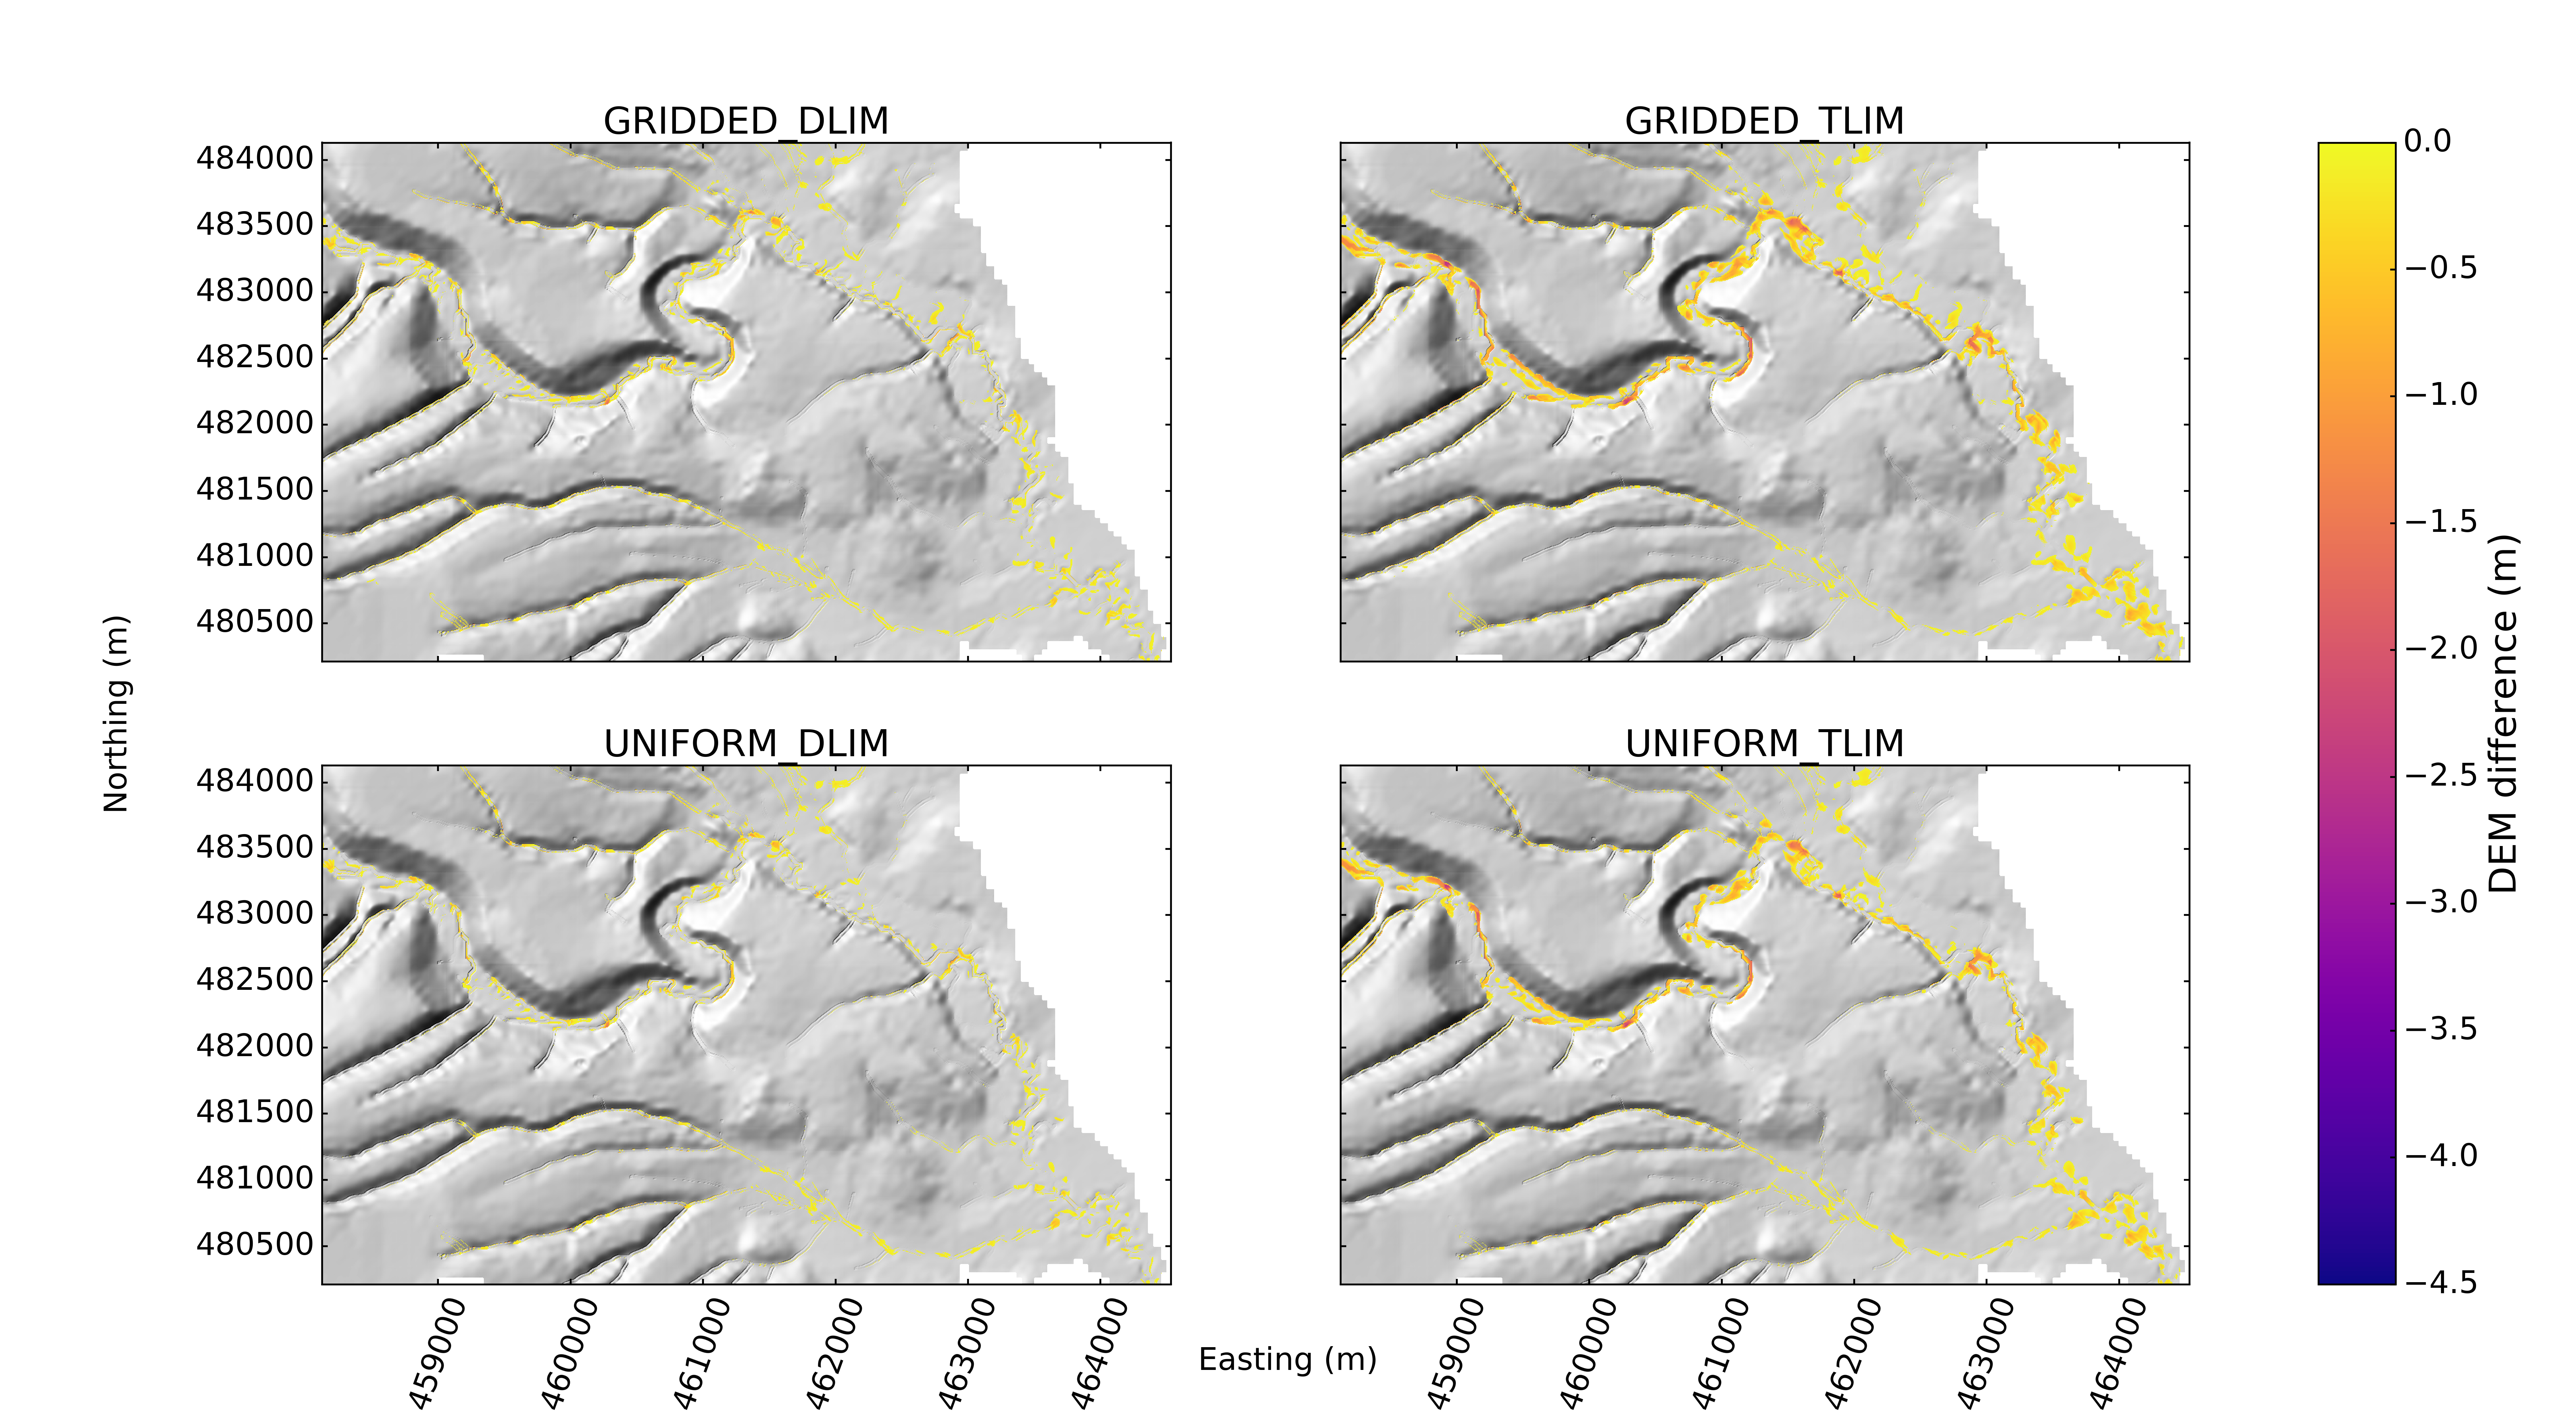
\includegraphics[width=25cm]{chp06_figures_scripts/figure_ryedale_erosion_diff_ensemble.png}
\caption{Ryedale. South-east section of Ryedale catchment showing the area around the village of Helmsley. Net difference in elevation after 72 hours simulation, showing the gridded and uniform rainfall simulations, for each of the two erosion law end-members (transport-limited and detachment-limited). Elevation change smaller than \(\pm\) 0.2m in magnitude is not shown for clarity. }
\label{fig_ryedale_2dplan_erosion_ensemble}
\end{sidewaysfigure}

% Full extent erosion maps
\begin{sidewaysfigure}[t]
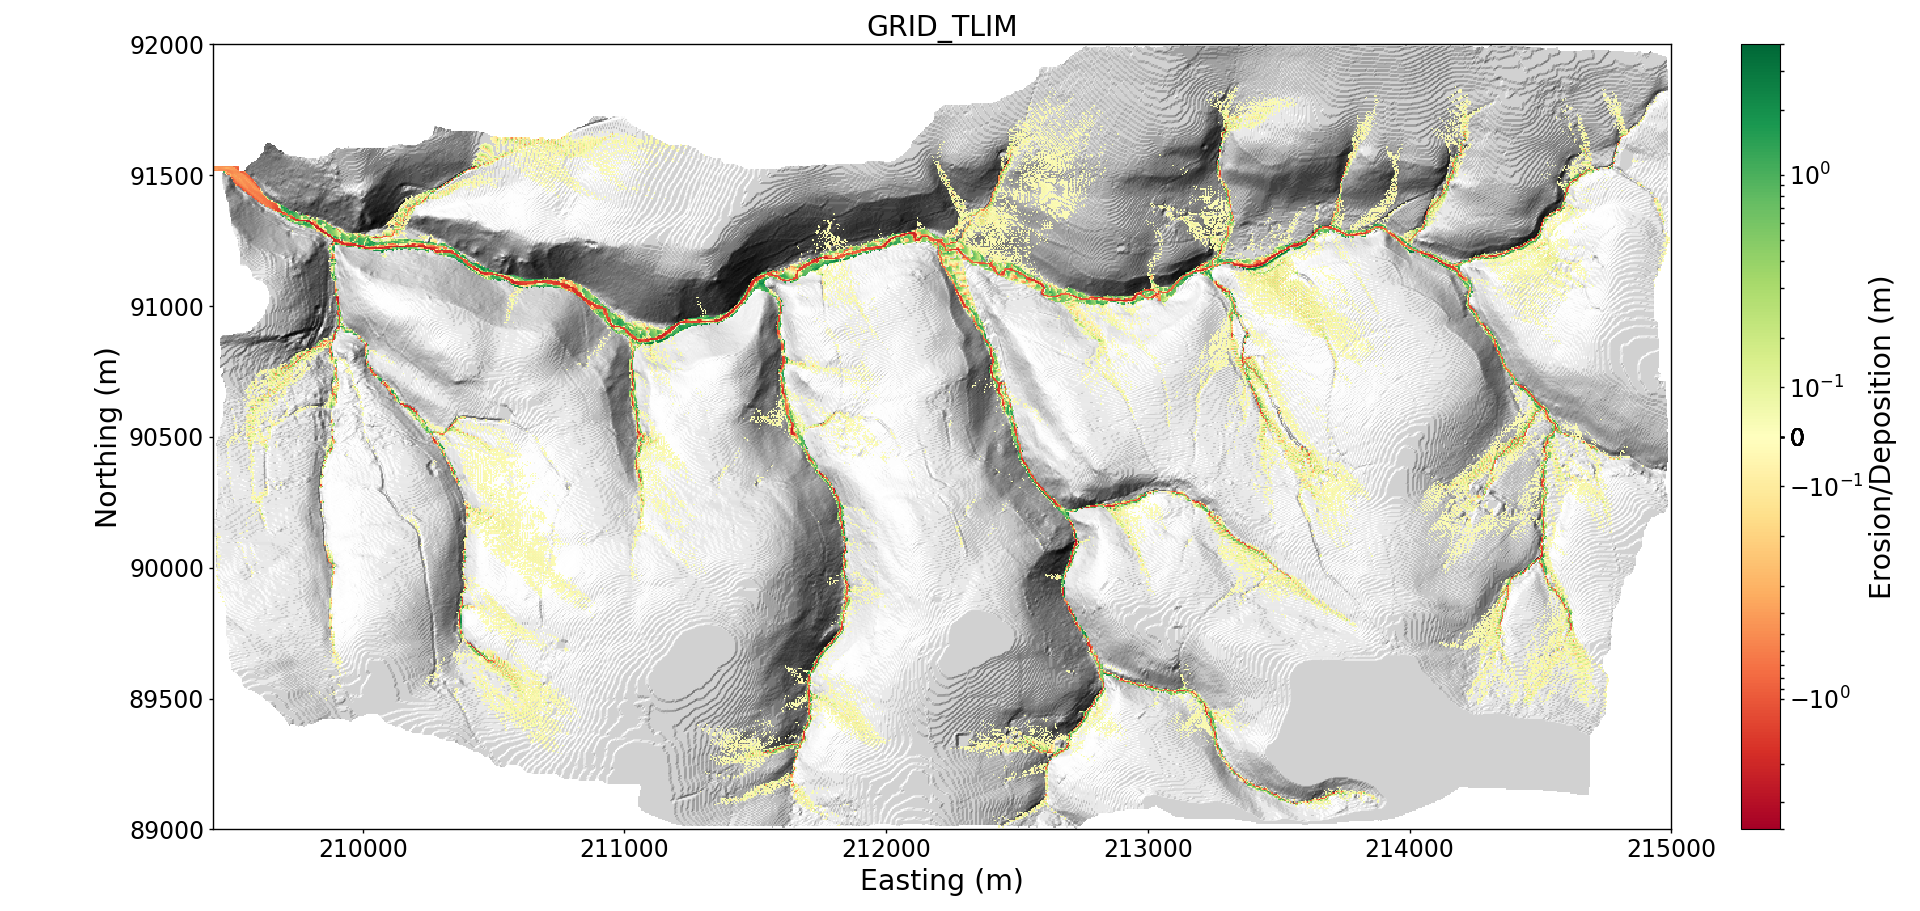
\includegraphics[width=25cm]{chp06_figures_scripts/boscastle_erodediff_grid_tlim.png}
\caption{Boscastle. Map of extent of catchment change in elevation greater than 0.02m. Change in elevation shown after 72 hours of model simulation using gridded rainfall and the transport limited erosion law. Output from the gridded rainfall input, transport-limited erosion simulatio(GRID\_TLIM). Logarithmic scale for erosion.}
\label{fig_boscastle_erodediff_grid_tlim}
\end{sidewaysfigure}

\begin{sidewaysfigure}[t]
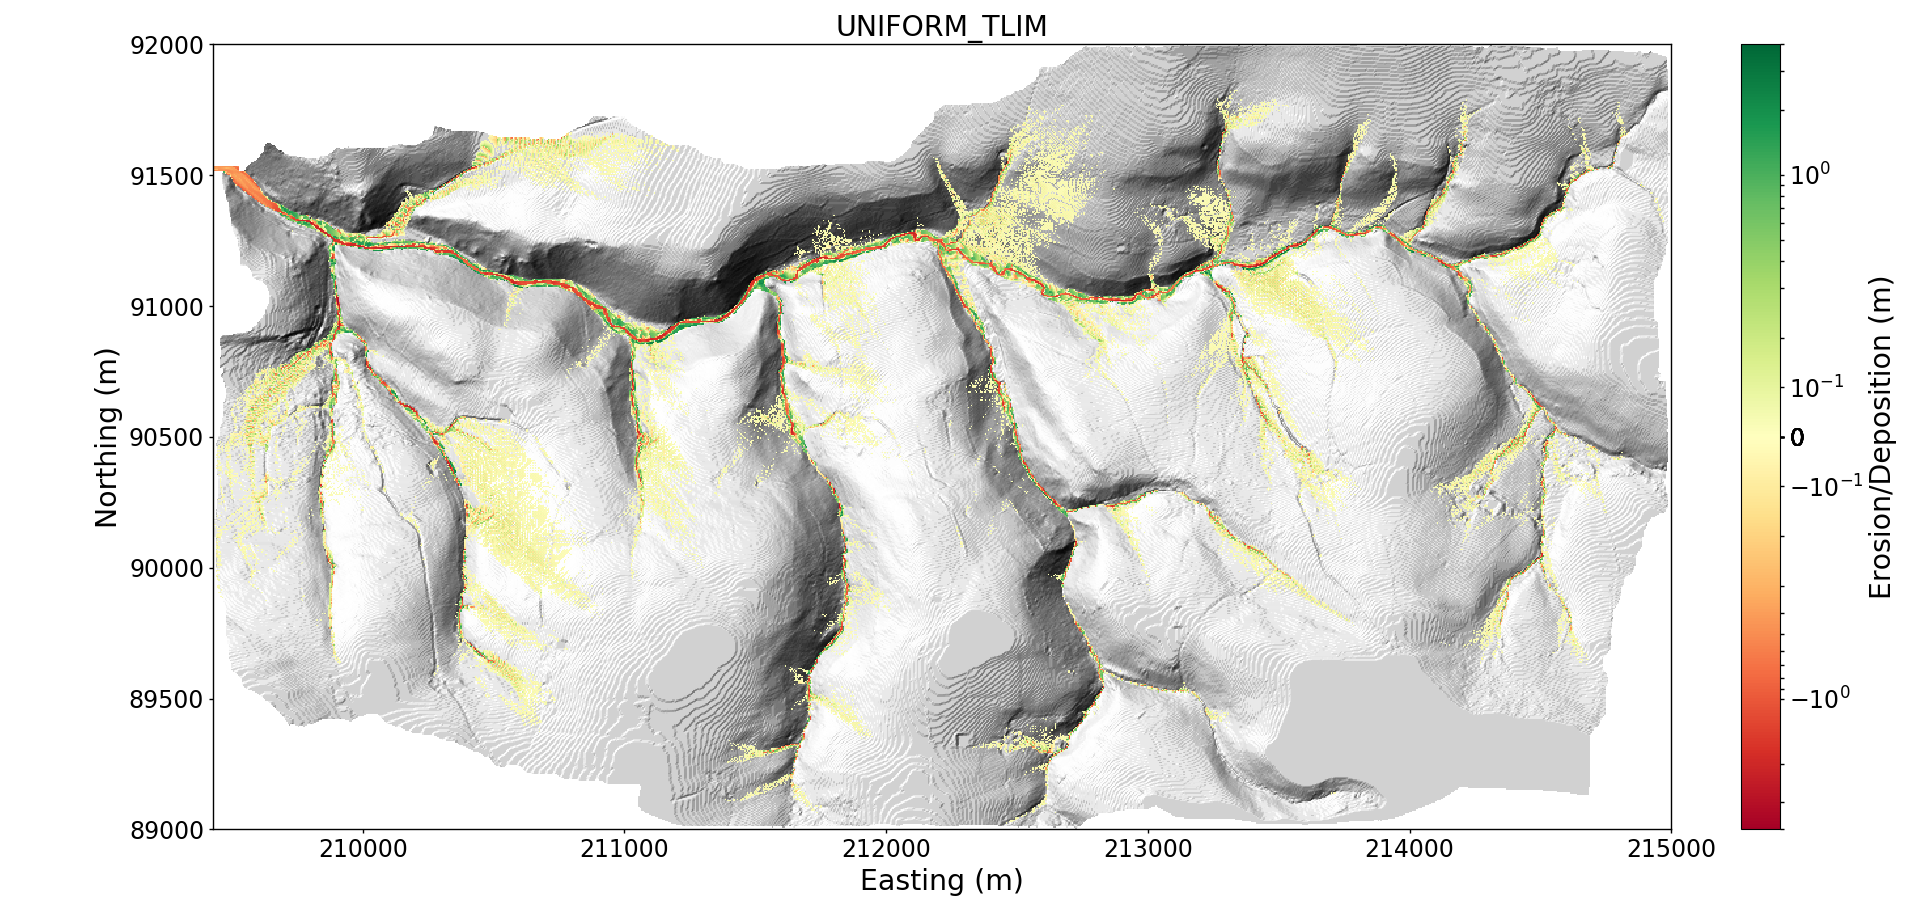
\includegraphics[width=25cm]{chp06_figures_scripts/boscastle_erodediff_uniform_tlim.png}
\caption{Boscastle. Map of extent of catchment change in elevation greater than 0.02m. Change in elevation shown after 72 hours of model simulation using uniform rainfall and the transport limited erosion law. Output from the uniform rainfall, transport-limited simulation (UNIFORM\_TLIM). Logarithmic scale for erosion.}
\label{fig_boscastle_erodediff_uniform_tlim}
\end{sidewaysfigure}

\begin{figure}[t]
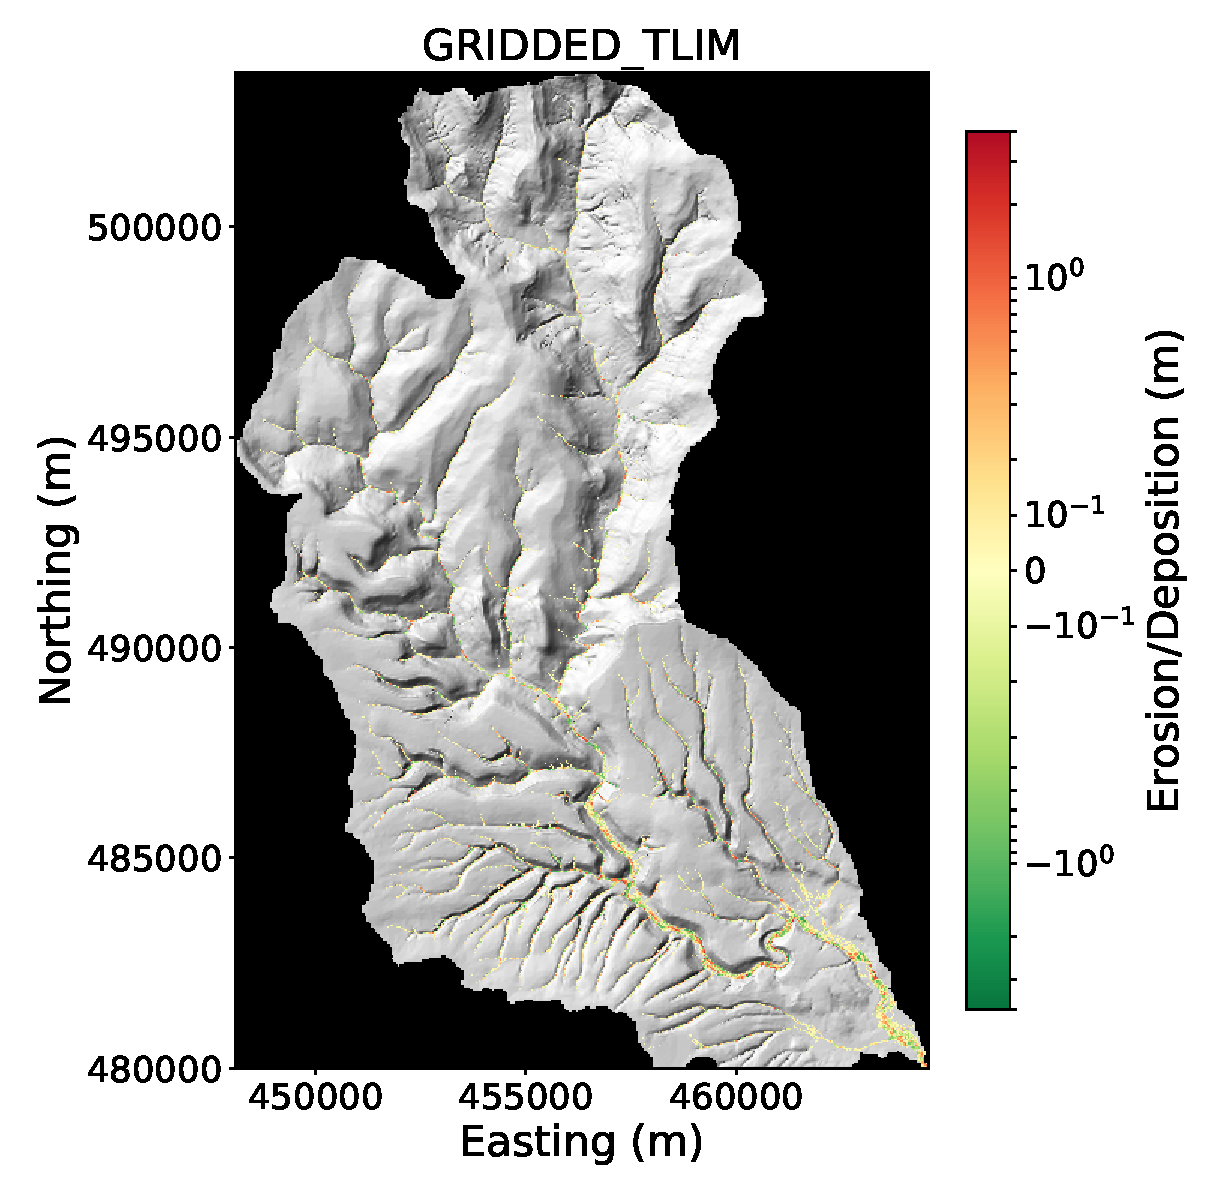
\includegraphics[width=16cm]{chp06_figures_scripts/figure_ryedale_elev_diff_grid_tlim.eps}
\caption{Ryedale. Map of extent of catchment change in elevation greater than 0.02m. Change in elevation shown after 72 hours of model simulation using uniform rainfall and the transport limited erosion law. Output from the uniform rainfall, transport-limited simulation (GRIDDED\_TLIM). Logarithmic scale for erosion.}
\label{fig_ryedale_erodediff_gridded_tlim}
\end{figure}

% RYEDALE lower reaches
%\begin{figure}[htb]
%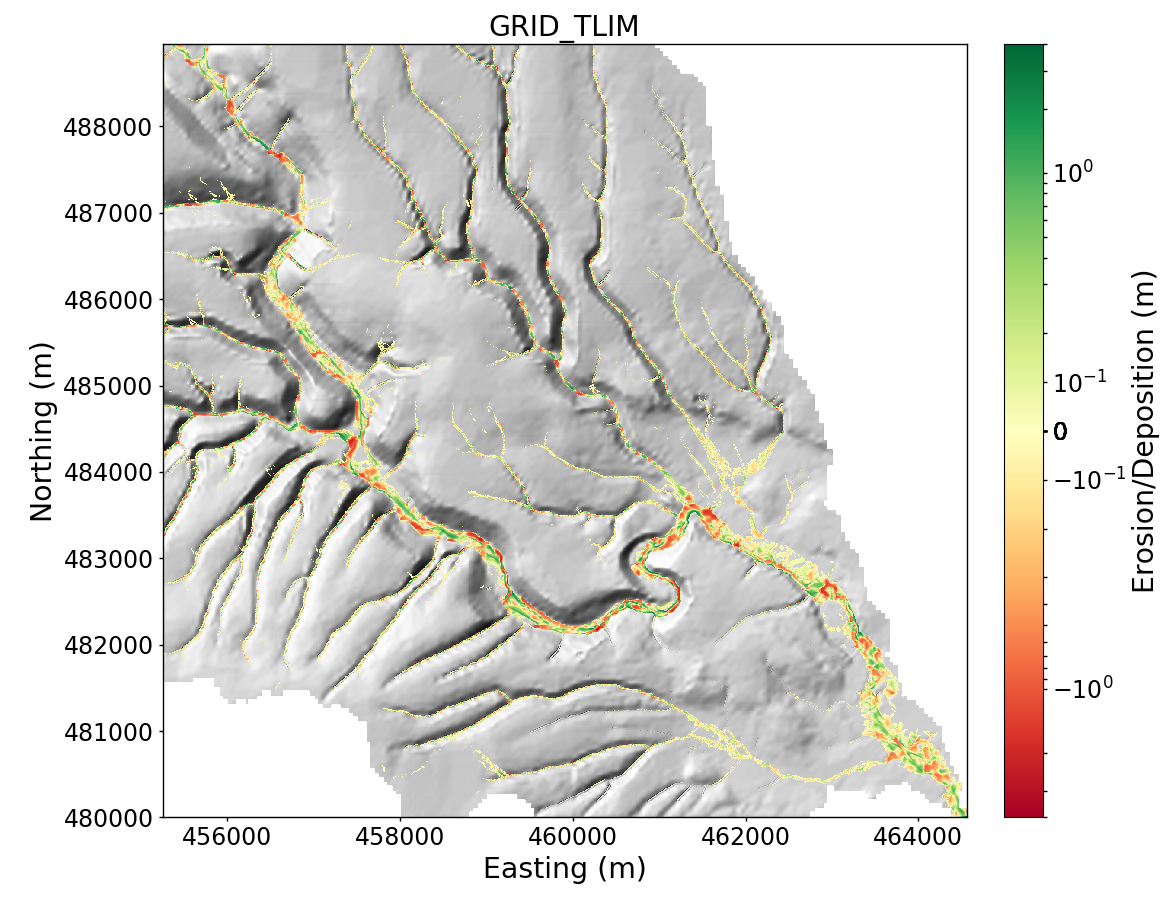
\includegraphics[width=16cm]{chp06_figures_scripts/fig_ryedale_lower_erodediff_grid_tlim.png}
%\caption{Ryedale. Map of extent of catchment change in elevation greater than 0.02m. Change in elevation shown after 72 hours of model simulation using gridded rainfall and the transport limited erosion law. Output from the gridded rainfall input, transport-limited erosion simulation (GRIDDED\_TLIM). Logarithmic scale for erosion.}
%\label{fig_ryedale_erodediff_lower_grid_tlim}
%\end{figure}
%
%\begin{figure}[htb]
%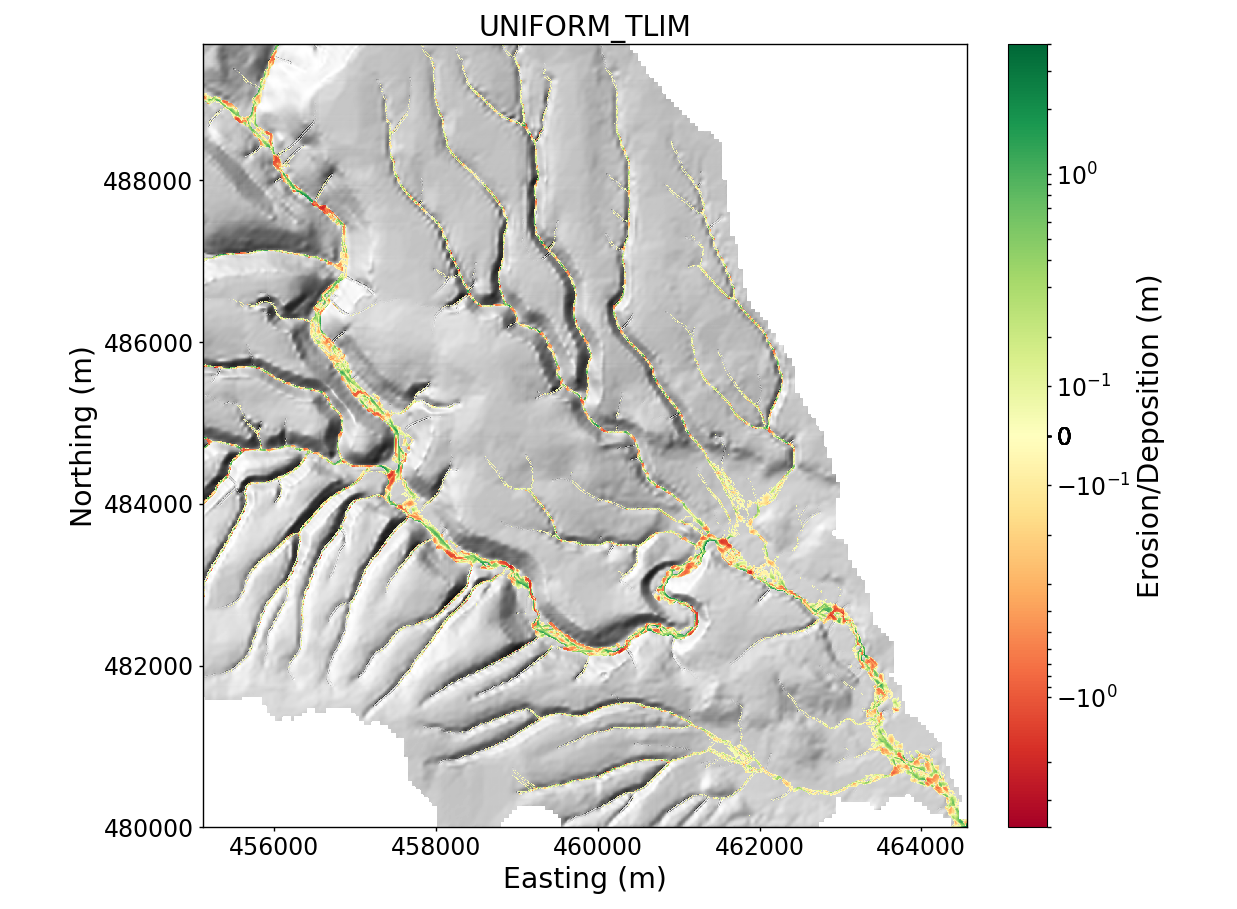
\includegraphics[width=16cm]{chp06_figures_scripts/fig_ryedale_lower_erodediff_uniform_tlim.png}
%\caption{Ryedale. Map of extent of catchment change in elevation greater than 0.02m. Change in elevation shown after 72 hours of model simulation using uniform rainfall and the transport limited erosion law. Output from the uniform rainfall, transport-limited simulation (UNIFORM\_TLIM). Logarithmic scale for erosion.}
%\label{fig_ryedale_erodediff_lower_uniform_tlim}
%\end{figure}

\begin{figure}[htb]
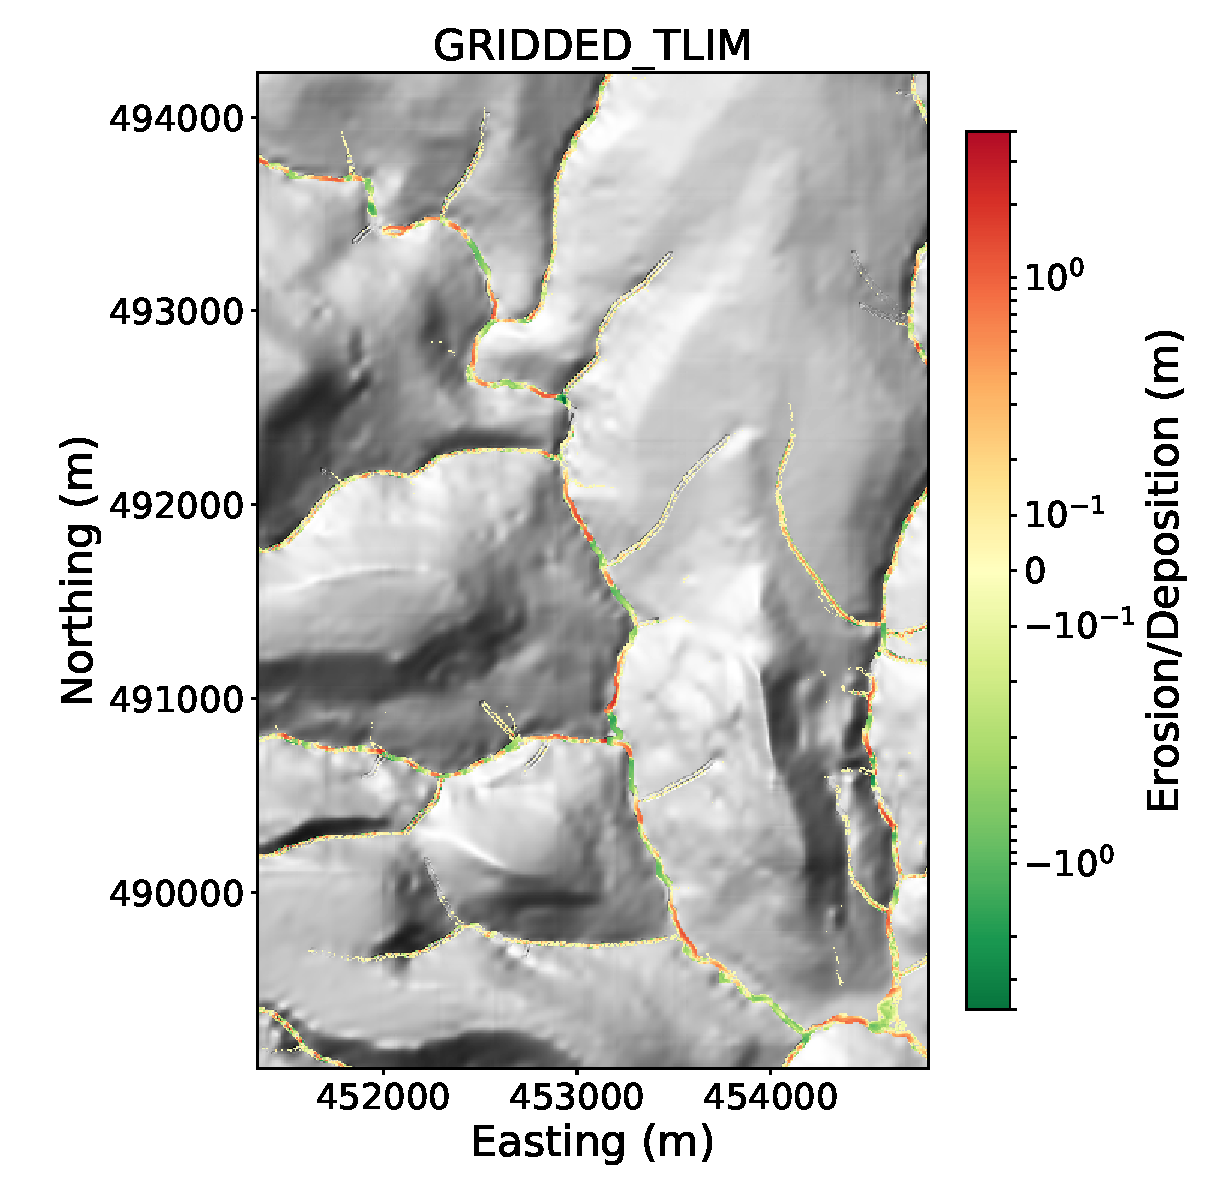
\includegraphics[width=16cm]{chp06_figures_scripts/figure_ryedale_elev_diff_grid_tlim_UPPER.eps}
\caption{Ryedale, upper Rye channel. Map of extent of erosion and deposition greater than 0.02m in magnitude. Change in elevation shown after 72 hours of model simulation using gridded rainfall and the transport-limited erosion law (\texttt{GRIDDED\_TLIM}). Logarithmic scale for erosion.}
\label{fig_ryedale_erodediff_UPPER_gridded_tlim}
\end{figure}

\begin{figure}[htb]
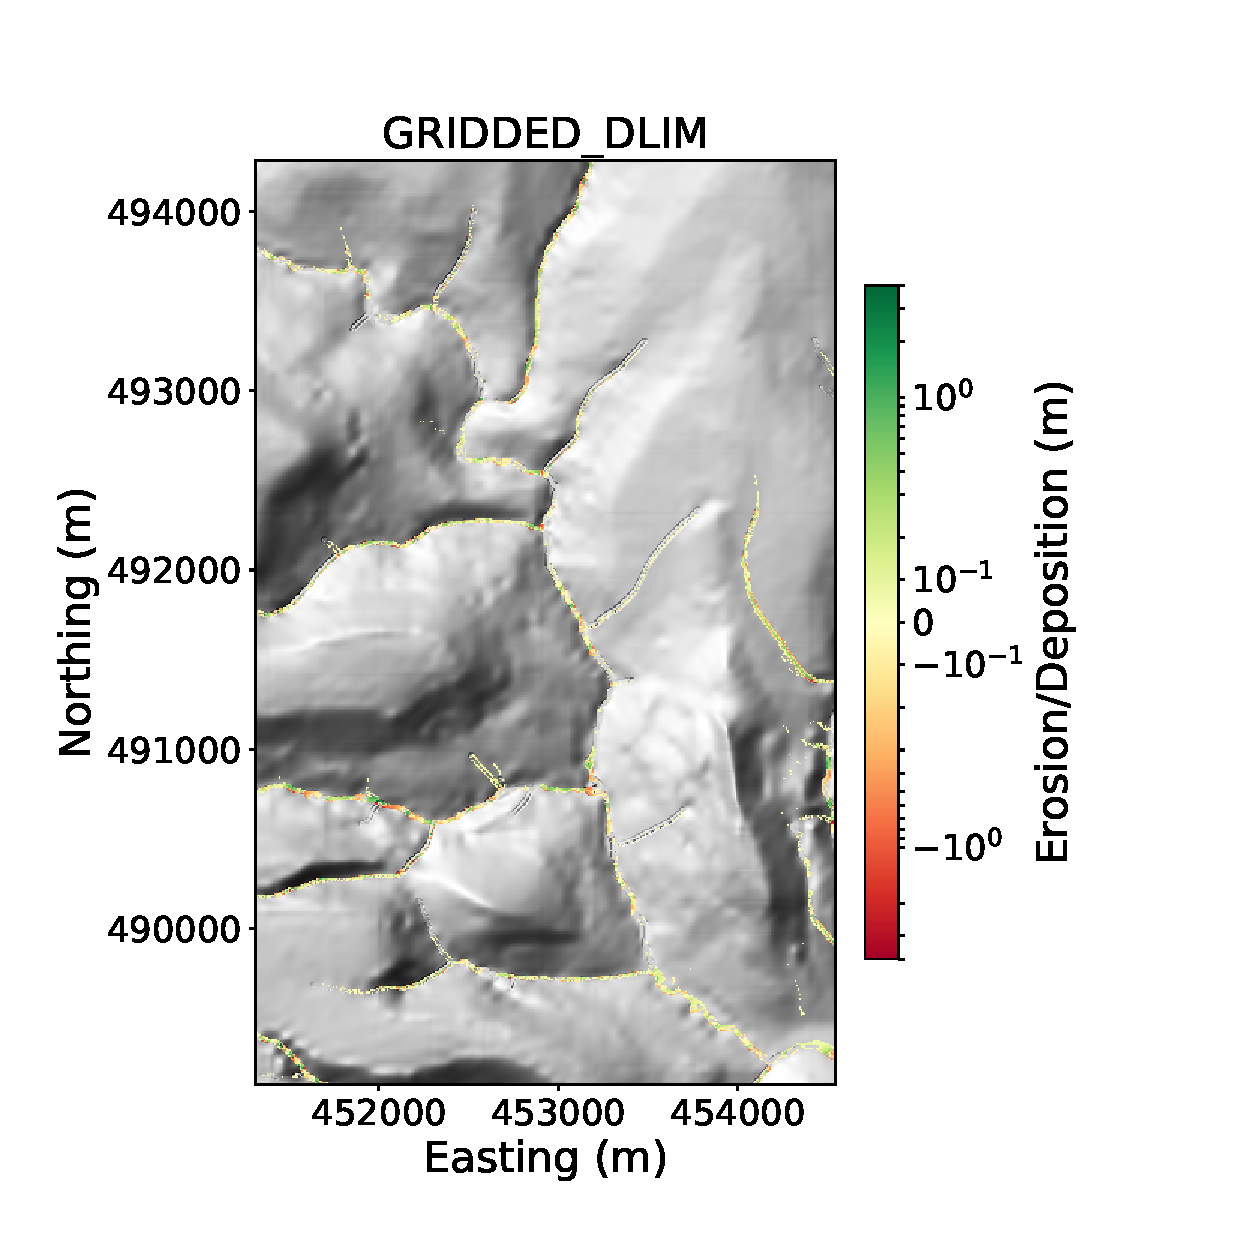
\includegraphics[width=16cm]{chp06_figures_scripts/figure_ryedale_elev_diff_grid_dlim_UPPER.eps}
\caption{Ryedale, upper Rye channel. Map of extent of erosion and deposition greater than 0.02m in magnitude. Change in elevation shown after 72 hours of model simulation using gridded rainfall and the detachment-limited erosion law (\texttt{GRIDDED\_DLIM}). Logarithmic scale for erosion.}
\label{fig_ryedale_erodediff_UPPER_gridded_dlim}
\end{figure}

\section{Discussion}

% Broader context of results
The relationship between the spatial distribution of rainfall and the erosional response of a river catchment has yet to be thoroughly explored. The analysis presented in this section discusses how erosional processes are sensitive to the spatial detail of precipitation in the context of flash flood events from intense rainfall. Improving our understanding of the relationship between rainfall patterns and erosional processes has two beneficiaries: 1) The short term environmental forecasting community will be able to better assess the role that  rainfall distribution has on sediment dynamics and erosion patterns. In the absence of spatially variable input data for environmental prediction, modellers will at least be able to gauge the potential uncertainty involved in sediment flux predictions and the distribution of erosion. 2) Within the context of longer term landscape evolution, this study contributes to understanding the importance of individual storm events in driving landscape change over geological timescales. Current parameterisation of rainfall heterogeneity in long term landscape evolution modelling is simplistic at best, and this results of this study can be used to guide rainfall parameterisation in landscape evolution model development. 

% Critical analysis of major findings.
The findings in this study are based on simulating historic flash flood events using a cellular automaton  landscape evolution numerical model, (HAIL-CAESAR, Chapter \ref{chapter_HAIL-CAESAR}). As such, the conclusions drawn from these experiments will be influenced by the individual characteristics of each catchment, though they were selected to be representative of typical upland catchments in the UK. Idiosyncrasies of the landscape evolution model, or simulation of different catchments and events may produce different outcomes, but the overall findings should be applicable to other similar modelling situations and catchment hydrogeomorphology in general.

\subsection{Sensitivity to erosion law and rainfall heterogeneity} 
One key finding from the experiments, exhibited in both case studies, is that erosion law choice in the model is a more dominant control on sediment flux, rather than the spatial detail of precipitation. The erosion-enabled simulations in these experiments represented two end-members of sediment transport and erosion laws (Table \ref{table_ensemble_experiments}): transport-limited and detachment-limited erosion. The transport-limited law simulations predict much greater sediment flux and erosion than their detachment-limited counterparts, with up to an order of magnitude of difference in places. In terms of sediment flux and erosion distribution, the role of rainfall input data spatial resolution played only a secondary role in determining erosion amounts. There was no clear evidence that the size of the catchment was found to be important in this respect, with even the smaller Boscastle catchment (18km\(^2\)) showing a marked sensitivity to the choice of erosion law and slight sensitivity to rainfall distribution. The sediment flux output from each catchment during the storm showed an order of magnitude difference between detachment and transport-limited erosion parameterisations, given the same rainfall spatial inputs. In contrast, the difference in sediment flux between uniform and gridded rainfall simulations was much smaller in both sets of simulations.

Despite this study showing choice of erosion law being the dominant factor in controlling sediment flux, the study does confirm previous reports of increased sediment outputs from simulations using spatially heterogeneous rainfall data to drive simulations. \citet{coulthard2016sensitivity} reported that using finer resolution rainfall data at 5km grid spacing (also derived from meteorological radar) resulted in a doubling of sediment yields from a similar sized upland catchment (415km\(^2\)). The key difference in their findings was that the result was observed after a much longer simulation time of 1000 years, using a 10-year rainfall record looped over the course of the 1000 year simulation. While the rainfall data used in \citet{coulthard2016sensitivity} contain maximum rainfall intensities approaching those observed in the Boscastle and Ryedale storms used here, it is not clear whether these rainfall peaks were part of prolonged storms over catchment, or were merely brief, localised cloudbursts. In other words, it cannot be determined whether the increase in sediment output observed in the \citet{coulthard2016sensitivity} gridded rainfall simulations is due to a particular storm in the 10 year rainfall record, due to cumulative erosive effects of lower intensity but higher frequency rainfall events, or some combination of both. The work presented in this chapter suggests that rainfall heterogeneity, while it may account for slightly higher sediment yields in individual storms, does not necessarily reproduce the 100\% differences observed in sediment yields over longer simulations such as in \citet{coulthard2016sensitivity}. However, this apparent discrepancy across timescales may be due to the specific characteristics of these particular storms studied -- other types of storm, different spatial distributions of rainfall, may be required to produce similar results to the \citet{coulthard2016sensitivity} study. 

\subsection{Comparison with observed geomorphic change post-flood}

The resulting geomorphic change from the Boscastle 2004 flood, and to a lesser extent, the Ryedale flood of 2005 were extensively surveyed in the aftermath of each event. Both sets of simulations lacked a suitably high-resolution DEM representing the state of the catchment before the flood took place, so a detailed before-and-after assessment of the accuracy of the model predictions is not possible. However, comparison with published reports on the erosion and deposition with each catchment allow us to make an assessment of whether the simulations were in broad agreement with the observations recorded after each flash flood event.

\subsubsection{Boscastle}
The geomorphological changes from the Boscastle flood were extensively mapped and recorded in an Environment Agency commissioned report carried out by \citet{wallingford2005flooding}. The amount of downcutting within the main Valency river channel was reported as 1--2m in places. The transport-limited simulations predicted  a similar magnitude of downcutting in places, but also tended to overestimate the amount of downcutting, predicting up to 4m in places, which was not confirmed at any location by the \citet{wallingford2005flooding} report . The detachment-limited simulations typically underestimated the amount of erosion and downcutting, particularly in the upper tributaries of the catchment, where little to no erosion was predicted, yet post-flood ground surveys reported substantial erosion within the channels. 

Substantial channel widening of up to 3--4m in places was reported in the HR Wallingford report. These simulations do not directly account for channel widening processes as there is no parameterisation of channel avulsion by lateral forces acting on the river bank within the HAIL-CAESAR model. The model allows indirect channel widening to take place through downcutting by water that has overtopped the channel banks, but this is not the primary mechanism through which channel widening occurs \citep{parker1976cause}. Future enhancements to the HAIL-CAESAR model would be needed to allow lateral channel widening to be investigated in the typical sense, similar to the implementations in \citet{murray1997properties,Coulthard2013}. The simulations presented in this chapter therefore do not fully reflect the channel widening reported in the post-flood geomorphological survey.

One area in which the gridded rainfall simulations performed better than the uniform rainfall inputs was in the tributaries in the south-east region of the catchment. The ground survey after the Boscastle flood noted significant amounts of erosion to in the tributaries on the south side of the Valency river. The tributary shown in Figure \ref{fig_boscastle_2dplan_erosion_ensemble_SE} was observed as having up to 1--2m of downcutting along its course. The gridded rainfall, transport-limited simulation \texttt{GRID\_TLIM} more accurately predicted this than the corresponding uniform rainfall input simulations. It is notable that the regions of the catchment with the highest rainfall input -- mainly the southern and eastern fringes of the catchment (Figure \ref{fig_boscastle_rain_totals}) -- fed into the tributaries that experienced the channel downcutting. In this particular case it is evidence that high resolution of rainfall input data can better resolve the pattern of erosion on the ground at a sub-catchment scale.

Deposition of sediment was observed along most sections of the lower reaches of the Valency floodplain. The transport-limited simulations predicted sediment deposition in the small floodplain areas immediately adjacent to he river channel, but substantially overpredicted the amount of sediment deposition in places, predicting as much as 2--3m of deposition. Ground surveys, while noting deposition of sediment in many places, reported sediment deposition on the order of centimetres, not metres. A similar overestimation of deposition was present in both the gridded and uniform rainfall simulations, reinforcing the conclusion that the choice and parameterisation of erosion law is a stronger controlling factor than the spatial heterogeneity of rainfall.

Large sediment deposits were recorded after the event in the harbour area of Boscastle village \citep{wallingford2005flooding}. Notably, all simulations failed to predict this correctly, in fact predicting net sediment erosion in the harbour area (Figure \ref{fig_boscastle_2dplan_erosion_ensemble}, north-west corner). The discord between observations and model predictions in the harbour area may arise from the poor parameterisation of the interface where the catchment drains out into the sea in this location. The sea and tide in the harbour act as a natural dampener to water flow velocities, which would be expected to encourage deposition of sediments here.

\subsubsection{Ryedale}

Geomorphic change in the aftermath of the Ryedale flood was not as extensively surveyed compared to the Boscastle event. However, several studies made qualitative and some quantitative observations regarding the geomorphic impact of the event \citep{dong2006evaluation,wass2008investigation,hopkins2012knowledge}.
Channel downcutting was substantial, with 2--3m reported in the upper tributaries of the Rye catchment \citep{wass2008investigation,hopkins2012knowledge}. This pattern of channel incision was generally captured in the transport-limited simulations of the Ryedale flood, but not in the detachment-limited simulations which tended to underpredict channel incision in the upper reaches of the catchment, which is shown in Figures \ref{fig_ryedale_erodediff_UPPER_gridded_dlim} and \ref{fig_ryedale_erodediff_UPPER_gridded_tlim}). Sediment deposition was reported in the lower reaches of the catchment, particularly in the village of Helmsley, but was not mapped extensively, unlike the Boscastle survey. The simulations show areas of sediment deposition and erosion on the orders of 0.5--3m around the Helmsley area and the surrounding flood plain. Photographic evidence \citep{dong2006evaluation,hopkins2012knowledge} however, suggests these predictions are somewhat over-estimates of the amount of incision and deposition in the floodplain area around Helmsley.

The Ryedale storm was noted for its triggering of over 100 shallow landslides within the catchment \citep{galiatsatos2007assessment,dong2006evaluation,
wass2008investigation}. The treatment of landsliding in the HAIL-CAESAR model is simplistic, based on a simple critical slope threshold required to trigger landslides, and as a result the reported landslides went largely unpredicted by all of the simulations. More complex models of landsliding are able to account for the role of soil saturation and pore water pressure in triggering of shallow landslides \citep[e.g.][]{iverson2000landslide,crosta2003distributed} and could be incorporated into future development of the model. 

\subsection{Implications for longer-term landscape evolution}
The experiments presented in this chapter have focused on the hydrogeomorphic response to single severe storm events, events which produced floods with return periods of 1 in 330 years (Ryedale) and 1 in 1300 years (Boscastle). The amounts of river channel incision predicted as a result of these storms is comparable to that predicted by studies of landscape evolution on scales of 1000 years, for example a study of a similar upland river basin by \citep{coulthard2016sensitivity} predicted channel incision amounts of 0.5--5m over a 1000 year simulation. Ground surveys after both events \citep{wallingford2005flooding,dong2006evaluation} revealed somewhat lower channel incision amounts, though of the same order of magnitude (1--3m). The transport-limited erosion law experiments presented here, using the same sediment transport law in the \citet{coulthard2016sensitivity} study, predict comparable amounts of channel incision during a single storm event. Previous studies of upland catchments in the UK that have experienced similar flash flood events have responded in a similar fashion \citep{johnson2002flooding,milan2012geomorphic}, showing catchment sediment fluxes far higher than typical background levels for similar sized catchments \citep[e.g.][]{johnson2002annual}. If the flood return periods are assumed to be broadly correct, these simulations, along with previously published field studies, support the view that the majority of sediment erosion occurs during infrequent but high magnitude flood events, rather than through gradual erosion or more frequent but lower magnitude events.

               
\subsection{Limitations}
The findings in this study are based on the outcomes of numerical simulations and data that are naturally simplifications of real landscapes and real rainfall events. Testing the potential for the HAIL-CAESAR model to forecast erosive episodes during flash flooding is limited due to the lack of pre- and post-event digital terrain models, therefore, only generalised conclusions can be made about the model's predictive ability when comparing the model output and the geomorphological surveys carried out after the events. 

A number of assumptions were made about the catchment, due in part to the complexity and number of environmental processes parameterised in the numerical model. Sediment transport processes are driven by the overland flow of water, and are therefore sensitive to the choice of hydrological and hydraulic parameters. Hydrological parameters such as the TOPMODEL \(m\) parameter, or Manning's \(n\) are difficult to determine without extensive field calibration. In this study, reported values of the TOPMODEL \(m\) parameter from previous studies in similar catchments were used as guidance \citep{beven1984testing,beven1997topmodel}, and in the case of the \(m\) parameter, sensitivity analysis was done (Chapter \ref{chapter_flood_model_sensitivity}) to determine the most appropriate value.   

Certain types of geomorphic change that were reported in post-event ground studies, such as channel avulsion in the Boscastle flood, and landsliding in the Ryedale event, are only simplistically represented in the HAIL-CAESAR model. The full range of catchment erosional processes, such as lateral river bank erosion and mass movement cannot yet be fully explored in terms of sensitivity to rainfall spatial distribution using this model alone. Nonetheless, the model captures the essential components of landscape evolution (overland flow and sediment transport by water) and their sensitivity to rainfall spatial distribution within a river catchment.


                       
\section{Conclusion}
This study was designed to test whether erosional processes in river catchments are sensitive to the spatial distribution of rainfall inputs, within the timeframe of an individual severe storm.
These experiments have shown that it is the choice of erosional parameterisation in the model, and not necessarily the spatial detail of rainfall input data, that has a first-order control on the total sediment yields from a catchment and the magnitude of river channel incision during a simulated event.

A further conclusion can also be made that rainfall spatial distribution does have an impact on sediment outputs and distribution of erosion in a catchment during an intense rainfall event, but in the cases shown here, it is a secondary control when compared to the choice and parameterisation of the erosion or sediment transport law. Where there is notable rainfall heterogeneity in a storm, spatially distributed rainfall data can be used to more accurately predict local variations in channel incision within the catchment, as was evident in the observed and predicted erosion patterns in the Boscastle catchment.

The study has touched upon whether landscape evolution models may be used for shorter-term forecasting tools to predict the impact of flash floods on the landscape, such as predicting local areas of channel erosion and deposition. There are still a number of limitations in current landscape erosion models that prevent them being used as tools of detailed predictive ability, notably the sensitivity from the choice of erosion laws as highlighted above. Using rainfall radar data as input to the model also introduces a further source of potential error (Chapter \ref{chapter_metdata}), which further compounds the uncertainty in predictions made by using a landscape evolution model in such a way to provide forecasts of landscape erosion in a single severe rainfall event. 

The importance of high magnitude, low frequency storm events as drivers of longer term landscape evolution is reinforced by this study. The amounts of channel incision predicted by the simulation (and confirmed in previously published geomorphological surveys), shows that a single storm can have as much erosive impact as centuries of higher frequency, lower magnitude events. If one were to extrapolate the differences in predictions between uniform and gridded rainfall inputs based on this study, the effect of rainfall spatial detail could be argued to play a secondary role on longer term landscape evolution. Cumulatively the small differences observed in erosion between uniform and gridded rainfall inputs to the model may become more pronounced over longer-term landscape evolution simulations, reconciling this study with previously published work. It is important to acknowledge that these findings are made in the context of individual events, and other factors and feedbacks may come into play over longer timescales. Nonetheless, the analysis of the numerical simulations presented in this chapter suggest that hydrogeomorphic process are at least partly sensitive to the spatial distribution of rainfall during intense storms.









